\section{Subgroups}

\subsection{Definitions and Examples}

\begin{exercise}
    In each of (a)-(e) prove that the specified subset is a subgroup of the given group:
    \begin{subproblems}
        \item the set of complex numbers of the form $a + ai$, $a \in \mathbb{R}$ (under addition)
        \item the set of complex numbers of absolute value $1$, i.e., the unit circle in the complex plane (under multiplication)
        \item for fixed $n \in \mathbb{Z}^+$ the set of rational numbers whose denominators divide $n$ (under addition)
        \item for fixed $n \in \mathbb{Z}^+$ the set of rational numbers whose denominators are relatively prime to $n$ (under addition)
        \item the set of nonzero real numbers whose square is a rational number (under multiplication)
    \end{subproblems}
\end{exercise}

\begin{sol}
    Let $G$ be the group and $H$ be the subset in equestion.
    \begin{subproblems}
        \item Since $0 + 0i \in H$, then $H$ is nonempty. For $a + ai, b + bi \in H$,
        \[(a + ai) - (b + bi) = (a - b) + (a - b)i \in H\]
        so that $H \leq G$.
        \item Since $\abs 1 = 1$, then $1 \in H$ so that it is nonempty. For $z, w \in H$, we first note that $|w\inv| = |\bar w|/|w|^2 = 1/1 = 1$, where $\bar w$ is the complex conjugate of $w$. Then
        \[|zw\inv| = |z||w\inv| = 1 \cdot 1 = 1\]
        so that $zw\inv \in H$, hence $H \leq G$.
        \item Fix $n \in \zp$. Since $0 = 0/k$ for some $k$ such that $k \mid n$, then $0 \in H$ so that $H$ is nonempty. Let $a/b, c/d \in H$ such that $(a, c) = (b, d) = 1$, and $b \mid n$ and $d \mid n$. Then there exists $x, y \in \zp$ such that $bx = n$ and $dy = n$. Then
        \[\frac ab - \frac cd = \frac{ax - cy}{n}\]
        where reducing this fraction still yields a denominator that divides $n$. Then $H \leq G$.
        \item Fix $n \in \zp$. Since $0 = 0/k$ for some $k$ such that $(k, n) = 1$, then $0 \in H$ so that $H$ is nonempty. Let $a/b, c/d \in H$ such that $(a, c) = 1$, $(b, n) = 1$, and $(d, n) = 1$. Then
        \[\frac ab - \frac cd = \frac{ad - bc}{bd}\]
        Assume, by way of contradiction, that $(bd, n) \neq 1$. Then there exists some prime $p$ such that $p \mid bd$ and $p \mid n$. Then $p \mid b$ or $p \mid d$, contradicting our assumption. Then $(bd, n) = 1$ so that $H \leq G$.
        \item Since $1 = 1^1 = 1/1$, then $1 \in H$ so that $H$ is nonempty. For $x, y \in H$, then $x^2, y^2 \in \q$. Then
        \[\left(\frac xy\right)^2 = \frac{x^2}{y^2} \in \q\]
        so that $x/y \in H$, hence $H \leq G$. \qh
    \end{subproblems}
\end{sol}

\newpage

\begin{exercise}
    In each of (a)--(e) prove that the specified subset is \emph{not} a subgroup of the given group:
    \begin{subproblems}
        \item the set of $2$-cycles in $S_n$ for $n \ge 3$
        \item the set of reflections in $D_{2n}$ for $n \ge 3$
        \item for $n$ a composite integer $>1$ and $G$ a group containing an element of order $n$, the set $\{x \in G \mid |x| = n\} \cup \{1\}$
        \item the set of (positive and negative) odd integers in $\mathbb{Z}$ together with $0$
        \item the set of real numbers whose square is a rational number (under addition)
    \end{subproblems}
\end{exercise}

\begin{sol}
    Let $G$ be the group and $H$ be the subset in question.
    \begin{subproblems}
        \item For $n = 3$, then $(1\ 2), (1\ 3) \in H$, but $(1\ 2)(1\ 3) = (1\ 3\ 2) \not\in H$.
        \item For $n = 3$, then $s, sr \in H$, but $s(sr) = r \not\in H$.
        \item Let $n = ab$ for some $a, b \in \zp$ with $1 < a, b < n$. Let $x \in G$ with $\abs x = n$. Then $x \in H$ so that $x^a \in H$, but $(x^a)^b = x^n = 1$ implies that $|x^a| \leq b$ so that $x^a \not\in H$.
        \item Observe that $1 \in H$, but $1 + 1 = 2 \not\in H$.
        \item Observe that $\sqrt 2, \sqrt 3 \in H$, but
        \[(\sqrt 2 + \sqrt 3)^2 = 2 + 2\sqrt 6 + 3 \not\in \q\]
        so that $\sqrt 2 + \sqrt 3 \not\in H$. \qh
    \end{subproblems}
\end{sol}

\begin{exercise}
    Show that the following subsets of the dihedral group $D_8$ are actually subgroups:
    \begin{subproblems}
        \item $\{1, r^2, s, sr^2\}$
        \item $\{1, r^2, sr, sr^3\}$
    \end{subproblems}
\end{exercise}

\begin{solalph}
    \item 
    \[
    \begin{array}{c|cccc}
        \circ & 1 & r^2 & s & sr^2 \\
        \hline
        1 & 1 & r^2 & s & sr^2 \\
        r^2 & r^2 & 1 & sr^2 & s \\
        s & s & sr^2 & 1 & r^2 \\
        sr^2 & sr^2 & s & r^2 & 1
    \end{array}
    \]
    \item 
    \[
    \begin{array}{c|cccc}
        \circ & 1 & r^2 & sr & sr^3 \\
        \hline
        1 & 1 & r^2 & sr & sr^3 \\
        r^2 & r^2 & 1 & sr^3 & sr \\
        sr & sr & sr^3 & 1 & r^2 \\
        sr^3 & sr^3 & sr & r^2 & 1
    \end{array}
    \]
    Both tables show closure, since no product is an element outside of the subset.
\end{solalph}

\begin{exercise}
    Give an explicit example of a group $G$ and an infinite subset $H$ of $G$ that is closed under the group operation but is not a subgroup of $G$.
\end{exercise}

\begin{sol}
    Let $G = \z$ and $H = \zp$. Then for any $m, n \in \zp$, we have $m + n \in \zp$ but $m - n \not\in \zp$ when $m < n$. Hence, $H$ is not a subgroup of $G$.
\end{sol}

\newpage

\begin{exercise}
    Prove that $G$ cannot have a subgroup $H$ with $|H| = n - 1$, where $n = |G| > 2$.
\end{exercise}

\begin{sol}
    Assume, by way of contradiction, that $G$ has a subgroup $H$ where $\abs H = n - 1$. By Lagrange's Theorem, $\abs H$ divides $\abs G$, so there exists some $k \in \zp$ such that $k(n - 1) = kn - k = n$, Equivalently, $n = k/(k - 1)$. Since $n > 2$, then $k > 2$. Then $k/(k - 1)$ is not an integer, a contradiction. Hence, no such subgroup $H$ exists.
\end{sol}

\begin{specialexercise} \label{ex2.1.6}
    Let $G$ be an abelian group. Prove that $\{ g \in G \mid |g| < \infty \}$ is a subgroup of $G$ (called the torsion subgroup of $G$). Give an explicit example where this set is not a subgroup when $G$ is non-abelian.
\end{specialexercise}

\begin{sol}
    Denote the set as $\tor(G)$. Since $\abs 1 = 1$, then $1 \in \tor(G)$ so that $\tor(G)$ is nonempty. Suppose $g, h \in \tor(G)$ where $\abs g = m$ and $\abs h = n$ for $m, n \in \zp$. Then
    \[(gh\inv)^{mn} = g^{mn}(h\inv)^{mn} = (g^m)^n((h^n)\inv)^m = 1^n(1\inv)^m = 1\]
    where we use the fact that $G$ is abelian to rearrange the terms. Then $\abs{gh\inv} \leq mn < \infty$ so that $gh\inv \in \tor(G)$, hence $\tor(G) \leq G$.

    For a non-abelian example, let $G = \aut(\r)$. Consider the elements $f, g \in G$ defined as $f(x) = -x$ and $g(x) = 1 - x$. Note that $\abs f = 2$ and $\abs g = 2$, but
    \[(fg)(x) = f(g(x)) = f(1 - x) = x - 1\]
    It is easy to show by induction that $(fg)^n(x) = x - n$ for all $n \in \zp$, so that $\abs{fg} = \infty$. Then $fg \not\in \tor(G)$, hence $\tor(G)$ is not a subgroup of $G$.
\end{sol}

\begin{exercise}
    Fix some $n \in \mathbb{Z}$ with $n>1$. Find the torsion subgroup (cf. the previous exercise) of $\mathbb{Z} \times (\mathbb{Z}/n\mathbb{Z})$. Show that the set of elements of infinite order together with the identity is \emph{not} a subgroup of this direct product.
\end{exercise}

\begin{sol}
    Observe that the only element of finite order in $\z$ is 0. Moreover, every element of $\intmod$ is of finite order. Then
    \[\tor(\z \times \intmod) = \set{(0, \bar x) \mid \bar x \in \intmod}\]
    Now consider the set of elements of infinite order together with the identity. Denoting this set as $H$, observe that $(1, 1), (-1, 0) \in H$, but
    \[(1, 1)(-1, 0) = (0, 1) \not\in H\]
    since $\abs{(0, 1)} = n < \infty$. Hence, $H$ is not a subgroup of $\z \times \intmod$.
\end{sol}

\begin{exercise}
    Let $H$ and $K$ be subgroups of $G$. Prove that $H \cup K$ is a subgroup if and only if either $H \subseteq K$ or $K \subseteq H$.
\end{exercise}

\begin{solitem}
    \item[\rightimp] Suppose $H \cup K$ is a subgroup. If $H \subseteq K$, then we are done. Suppose that $H \nsubseteq K$. Then there exists some $h \in H$ such that $h \not\in K$. Since $H \cup K$ is a subgroup, then for any $k \in K$, we have $hk \in H \cup K$.
    
    Observe that $k\inv \in K$ since $K \leq G$. If $hk \in K$, then $h = (hk)k\inv \in K$, contradicting our assumption. It must be that $hk \in H$. Since $h \in H$, then $h\inv H$ as $H \leq G$. Then $h\inv(hk) = k \in H$, hence $K \subseteq H$.
    \item[\leftimp] If $H \subseteq K$, then $H \cup K = K \leq G$. Similarly, if $K \subseteq H$, then $H \cup K = H \leq G$.
\end{solitem}

\begin{specialexercise} \label{ex2.1.9}
    Let $G = \gl_n(F)$, where $F$ is any field. Define
    \[\speclin_n(F) = \{ A \in \gl_n(F) \mid \det(A) = 1 \}\]
    (called the special linear group). Prove that $\speclin_n(F) \le \gl_n(F)$.
\end{specialexercise}

\begin{sol}
    Since $\det(I_n) = 1$, then $I_n \in \speclin_n(F)$ so that $\speclin_n(F)$ is nonempty. Suppose $A, B \in \speclin_n(F)$. Then
    \[\det(AB\inv) = \det(A)\det(B\inv) = \frac{\det(A)}{\det(B)} = \frac 11 = 1\]
    so that $AB\inv \in \speclin_n(F)$. It follows that $\speclin_n(F) \leq \gl_n(F)$.
\end{sol}

\begin{exercise} \label{ex2.1.10}
    \begin{subproblems}
        \item Prove that if $H$ and $K$ are subgroups of $G$ then so is their intersection $H \cap K$.
        \item Prove that the intersection of an arbitrary nonempty collection of subgroups of $G$ is again a subgroup of $G$ (do not assume the collection is countable).
    \end{subproblems}
\end{exercise}

\begin{solalph}
    \item Let $L = H \cap K$. Since $1 \in H$ and $1 \in K$ because $H \leq G$ and $K \leq G$, then $1 \in L$ so that $L$ is nonempty. Suppose $a, b \in L$. Then $a, b \in H$ and $a, b \in K$. Since $H$ and $K$ are subgroups of $G$, then $ab\inv \in H$ and $ab\inv \in K$. Hence, $ab\inv \in L$, and $L \leq G$.
    \item Let $I$ be an indexing set, and consider the collection of subgroups $\{ H_i \}_{i \in I}$ of $G$. Let
    \[H = \bigcap_{i \in I} H_i\]
    Since $1 \in H_i$ for all $i \in I$, then $1 \in H$. Suppose $a, b \in H$. Then $a, b \in H_i$ for all $i \in I$. Since each $H_i$ is a subgroup of $G$, then $ab\inv \in H_i$ for all $i \in I$. Hence, $ab\inv \in H$, and $H \leq G$.
\end{solalph}

\begin{exercise}
    Let $A$ and $B$ be groups. Prove that the following sets are subgroups of the direct product $A \times B$:
    \begin{subproblems}
        \item $\{ (a, 1) \mid a \in A \}$
        \item $\{ (1, b) \mid b \in B \}$
        \item $\{ (a, a) \mid a \in A \}$, where we assume $B = A$ (called the diagonal subgroup)
    \end{subproblems}
\end{exercise}

\begin{sol}
    Let $C$ be the set in each part.
    \begin{subproblems}
        \item Since $1 \in A$, then $(1, 1) \in C$ so that $C$ is nonempty. Suppose $(a_1, 1), (a_2, 1) \in C$. Then
        \[(a_1, 1)(a_2, 1)\inv = (a_1, 1)(a_2\inv, 1) = (a_1a_2\inv, 1) \in C\]
        since $a_1a_2\inv \in A$. Hence, $C \leq A \times B$.
        \item Since $1 \in B$, then $(1, 1) \in C$ so that $C$ is nonempty. Suppose $(1, b_1), (1, b_2) \in C$. Then
        \[(1, b_1)(1, b_2)\inv = (1, b_1)(1, b_2\inv) = (1, b_1b_2\inv) \in C\]
        since $b_1b_2\inv \in B$. Hence, $C \leq A \times B$.
        \item Since $1 \in A$, then $(1, 1) \in C$ so that $C$ is nonempty. Suppose $(a_1, a_1), (a_2, a_2) \in C$. Then
        \[(a_1, a_1)(a_2, a_2)\inv = (a_1, a_1)(a_2\inv, a_2\inv) = (a_1a_2\inv, a_1a_2\inv) \in C\]
        since $a_1a_2\inv \in A$. Hence, $C \leq A \times B$. \qh
    \end{subproblems}
\end{sol}

\begin{exercise}
    Let $A$ be an abelian group and fix some $n \in \mathbb{Z}$. Prove that the following sets are subgroups of $A$:
    \begin{subproblems}
        \item $\{ a^n \mid a \in A \}$
        \item $\{ a \in A \mid a^n = 1 \}$
    \end{subproblems}
\end{exercise}

\begin{sol}
    Let $B$ be the sets in question.
    \begin{subproblems}
        \item Since $1 = 1^n$, then $1 \in B$ so that $B$ is nonempty. Suppose $a^n, b^n \in B$. Then
        \item \[(a^n)(b^n)\inv = a^n b^{-n} = (ab\inv)^n \in B\]
        where the last equality follows from the fact that $A$ is abelian. Hence, $B \leq A$.
        \item Since $1^n = 1$, then $1 \in B$ so that $B$ is nonempty. Suppose $a, b \in B$. Then
        \[(ab\inv)^n = a^n (b\inv)^n = a^n (b^n)\inv = 1 \cdot 1\inv = 1\]
        where the second equality follows from the fact that $A$ is abelian. Hence, $B \leq A$. \qh
    \end{subproblems}
\end{sol}

\begin{exercise}
    Let $H$ be a subgroup of the additive group of rational numbers with the property that $1/x \in H$ for every nonzero element $x$ of $H$. Prove that $H = 0$ or $\mathbb{Q}$.
\end{exercise}

\begin{sol}
    Let $H \leq \q$. Then $0 \in H$. If no other elements are in $H$, then $H = 0$, and we are done. Suppose there exists some nonzero $a/b \in H$ where $a, b \in \z$ and $b \neq 0$. Moreover, we may assume without loss of generality that $a/b > 0$, for otherwise we may take $-a/b$ since $H$ contains additive inverses. We now use $a/b$ to generate $\q$.

    Since $a/b \in H$, then $b(a/b) = a \in H$ so that $1/a \in H$. Then $a(1/a) = 1 \in H$. From this, we can see that $\z \subseteq H$. Now let $c/d \in \q$ for some $c, d \in \z$ with $d \neq 0$. Since $1 \in H$, then $d(1) = d \in H$ so that $1/d \in H$. Then $c(1/d) = c/d \in H$. Since $c/d$ was arbitrary, then $\q \subseteq H$. Hence, $H = \q$.
\end{sol}

\begin{exercise}
    Show that $\{ x \in D_{2n} \mid x^2 = 1 \}$ is \emph{not} a subgroup of $D_{2n}$ (here $n \ge 3$).
\end{exercise}

\begin{sol}
    Let $H$ be the set in question. Clearly, $s \in H$. Moreover,
    \[(sr)^2 = srsr = ssr\inv r = 1\]
    so that $|sr| = 2$ and $sr \in H$. However, $s(sr) = r \not\in H$ since $\abs r = n > 2$. Hence, $H$ is not a subgroup of $D_{2n}$.
\end{sol}

\begin{exercise}
    Let $H_1 \subseteq H_2 \subseteq \cdots$ be an ascending chain of subgroups of $G$. Prove that $\bigcup_{i=1}^\infty H_i$ is a subgroup of $G$.
\end{exercise}

\begin{sol}
    Let
    \[H = \bigcup_{i=1}^\infty H_i\]
    Since $H_i \leq G$ for each $i \in \zp$, then $1 \in H_i$ for all $i \in \zp$, hence $1 \in H$ so that $H$ is nonempty. Suppose $a, b \in H$. Then there exists some $m, n \in \zp$ such that $a \in H_m$ and $b \in H_n$. Let $k = \max(m, n)$. Since $H_m \subseteq H_k$ and $H_n \subseteq H_k$, then $a, b \in H_k$. Since $H_k \leq G$, then $ab\inv \in H_k$, hence $ab\inv \in H$. It follows that $H \leq G$.
\end{sol}

\newpage

\begin{specialexercise}
    Let $n \in \mathbb{Z}^+$ and let $F$ be a field. Prove that the set $\{ (a_{ij}) \in \gl_n(F) \mid a_{ij} = 0 \text{ for all } i > j \}$ is a subgroup of $\gl_n(F)$ (called the group of upper triangular matrices).
\end{specialexercise}

\begin{sol}
    Let $\ut_n(F)$ denote the set of $n \times n$ upper triangular matrices with entries from $F$. Observe that $I_n$ contains $0$'s everywhere except the diagonal, hence $I_n \in \ut_n(F)$ so that $\ut_n(F)$ is nonempty. Suppose $A, B \in \ut_n(F)$, and consider $C = AB$. Then the $(i, j)$-th entry of $C$ is given by
    \[c_{ij} = \sum_{k = 1}^n a_{ik}b_{kj}\]
    Consider the case when $i > j$, which is below the main diagonal.
    \begin{itemize}
        \item If $i > k$, then $a_{ik} = 0$ since $A$ is upper triangular.
        \item If $k > j$, then $b_{kj} = 0$ since $B$ is upper triangular.
    \end{itemize}
    Hence, for all $k$, either $a_{ik} = 0$ or $b_{kj} = 0$, so that $c_{ij} = 0$. It follows that $C \in \ut_n(F)$.

    Let $A \in \ut_n(F)$, and let $D \in \gl_n(F)$ such that $AD = DA = I_n$. We show by induction that $D \in \ut_n(F)$. For the base case, consider $n = 2$. Since we know $A \in \ut_n(F)$ by assumption but do not know about $D$, we write
    \[A =
    \begin{pmatrix}
        a_{11} & a_{12} \\
        0 & a_{22}
    \end{pmatrix}, \quad
    D =
    \begin{pmatrix}
        d_{11} & d_{12} \\
        d_{21} & d_{22}
    \end{pmatrix}, \quad
    AD = 
    \begin{pmatrix}
        a_{11} d_{11} + a_{12} d_{21} & a_{11} d_{12} + a_{12} d_{22} \\
        a_{22} d_{21} & a_{22} d_{22}
    \end{pmatrix} = I_2
    \]
    Observe that $a_{22}d_{21} = 0$. Since $a_{22} \neq 0$ because $A \in \ut_2(F) \subseteq \gl_2(F)$, then $d_{21} = 0$, hence $D \in \ut_2(F)$. Now suppose that the inverse of any upper triangular matrix in $\gl_n(F)$ is also upper triangular, and consider $A \in \ut_{n + 1}(F)$ and $D \in \gl_{n + 1}(F)$ such that $AD = DA = I_{n + 1}$. Using block matrices, we may write this as
    \[A = 
    \begin{pmatrix}
        A_0 & \b a_{12} \\
        0 & a_{22}
    \end{pmatrix}, \quad
    D = 
    \begin{pmatrix}
        D_0 & \b d_{12} \\
        \b d_{21}^T & d_{22}
    \end{pmatrix}, \quad
    AD = 
    \begin{pmatrix}
        A_0 D_0 & A_0 \b d_{12} + \b a_{12} d_{22} \\
        a_{22} \b d_{21}^T & a_{22} d_{22}
    \end{pmatrix} = I_{n + 1}
    \]
    where $\b a_{12}, \b d_{12}, \b d_{21}^T$ are $n \times 1$ column vectors, and $a_{22}, d_{22} \in F$. We can see that $A_0 D_0 = I_n$ so that $D_0 \in \ut_n(F)$ by assumption. Moreover, $a_{22} \b d_{21}^T = \b 0_{n \times 1}^T$. Since $a_{22} \neq 0$ because $A \in \ut_{n + 1}(F)$, then $\b d_{21}^T = \b 0_{n \times 1}^T$. By induction, then $D \in \ut_{n + 1}(F)$, hence the inverse of any upper triangular matrix is also upper triangular.
\end{sol}

\begin{exercise}
    Let $n \in \mathbb{Z}^+$ and let $F$ be a field. Prove that the set $\{ (a_{ij}) \in \gl_n(F) \mid a_{ij} = 0 \text{ for all } i > j,\ \text{and } a_{ii} = 1 \text{ for all } i \}$ is a subgroup of $\gl_n(F)$.
\end{exercise}

\begin{sol}
    Let $H$ be the set in question. Since the diagonal of $I_n$ is only 1's, then $I_n \in H$. Suppose $A, B \in H$. By the previous exercise, $A, B \in \ut_n(F)$, so it remains to show that $a_{ii} = b_{ii} = 1$ for all $1 \leq i \leq n$. Then
    \[(AB)_{ii} = \sum_{k = 1}^n a_{ik}b_{ki}\]
    Since $a_{ik} = 0$ for $k < i$ and $b_{ki} = 0$ for $k > i$, then the sum degrades to $a_{ii}b_{ii} = 1$. Then $H$ is closed under multiplication. Moreover, suppose $D \in \ut_n(F)$ such that $DA = I_n$. Then
    \[1 = (DA)_{ii} = d_{ii}a_{ii}\]
    where we use the above to collapse the $ii$-th term of $DA$. Then $d_{ii} = 1$, hence $D \in H$, and $H$ is closed under inverses. Hence, $H \leq \gl_n(F)$.
\end{sol}

\subsection{Centralizers and Normalizers, Stabilizers and Kernels}

\begin{exercise}
    Prove that $C_G(A)=\{g\in G\mid g^{-1}ag=a\text{ for all }a\in A\}.$
\end{exercise}

\begin{sol}
    For any $a \in A \subseteq G$, then $g \in C_G(A)$ if and only if $gag\inv = a$ if and only if $ga = ag$ if and only if $g\inv ag = a$. Hence, $C_G(A) = \{g \in G \mid g\inv ag = a \text{ for all } a \in A\}$.
\end{sol}

\begin{exercise}
    Prove that $C_G(Z(G))=G$ and deduce that $N_G(Z(G))=G.$
\end{exercise}

\begin{sol}
    By definition, $C_G(Z(G)) \subseteq G$. Now let $g \in G$ and $z \in Z(G)$. Then $gz = zg$, or $gzg\inv = z$. Then $g \in C_G(Z(G))$, hence $G \subseteq C_G(Z(G))$. It follows that $C_G(Z(G)) = G$. Since $C_G(Z(G)) \leq N_G(Z(G)) \leq G$, then $N_G(Z(G)) = G$.
\end{sol}

\begin{exercise}
    Prove that if $A$ and $B$ are subsets of $G$ with $A \subseteq B$ then $C_G(B)$ is a subgroup of $C_G(A)$.
\end{exercise}

\begin{sol}
    Pick $g \in C_G(B)$. Then $gbg\inv = b$ for all $b \in B$. In particular, $gag\inv = a$ for all $a \in A$ because $A \subseteq B$. Then $C_G(B) \subseteq C_G(A)$. Since $C_G(B)$ and $C_G(A)$ are subgroups of $G$, then $C_G(B) \leq C_G(A)$.
\end{sol}

\begin{specialexercise}
    For each of $S_3$, $D_8$, and $Q_8$ compute the centralizers of each element and find the center of each group. Does Lagrange's Theorem (\hyperref[ex1.7.19]{Exercise 1.7.19}) simplify your work?
\end{specialexercise}

\begin{sol}
    To compute the center of a group $G$, we need to compute the centralizer of each element in $G$ and then take the intersection of all these centralizers. The proof of this is trivial.

    We begin with $S_3$. It is trivial to see that $C_G(1) = G$ for any group $G$, since $1$ commutes with every element of $g$. Now consider $(1\ 2) \in S_3$, and consider the subgroup $A = \set{1, (1\ 2)}$. Since $A$ is a subgroup, then $A \leq C_{S_3}((1\ 2))$. By Lagrange's Theorem, then 2 divides $|C_{S_3}((1\ 2))|$ and $|C_{S_3}((1\ 2))|$ divides 6. Since $(1\ 3)(1\ 2) = (1\ 2\ 3) \neq (1\ 3\ 2) = (1\ 2)(1\ 3)$, then $(1\ 3) \not\in C_{S_3}((1\ 2))$. By \hyperref[ex1.3.20]{Exercise 1.3.20}, we know that $(1\ 2)$ and $(1\ 3)$ generate $S_3$ so that $|C_{S_3}((1\ 2))| \neq 6$. Then $|C_{S_3}((1\ 2))| = 2$ so that $C_{S_3}((1\ 2)) = A$. By symmetry, the same argument holds for $(1\ 3)$ and $(2\ 3)$, so that
    \[C_{S_3}((1\ 3)) = \set{1, (1\ 3)}, \quad C_{S_3}((2\ 3)) = \set{1, (2\ 3)}\]
    Now consider $(1\ 2\ 3) \in S_3$, and the subgroup $B = \set{1, (1\ 2\ 3), (1\ 3\ 2)}$. Since $B$ is a subgroup, then $B \leq C_{S_3}((1\ 2\ 3))$. By Lagrange's Theorem, then 3 divides $|C_{S_3}((1\ 2\ 3))|$ and $|C_{S_3}((1\ 2\ 3))|$ divides 6. Observe that $(1\ 2) \not\in C_{S_3}((1\ 2\ 3))$ since $(1\ 2)(1\ 2\ 3) \neq (1\ 2\ 3)(1\ 2)$. Then $|C_{S_3}((1\ 2\ 3))| \neq 6$, so that $|C_{S_3}((1\ 2\ 3))| = 3$ and $C_{S_3}((1\ 2\ 3)) = B$. By symmetry, the same argument holds for $(1\ 3\ 2)$. Moreover, $Z(G) = \set 1$.
    
    The following are the centralizers for each element in $D_8$:
    \begin{align*}
        C_{D_8}(1) & = D_8 & C_{D_8}(r) & = \set{1, r, r^2, r^3} \\
        C_{D_8}(r^3) & = \set{1, r, r^2, r^3} & C_{D_8}(r^2) & = D_8 \\
        C_{D_8}(sr) & = \set{1, r^2, sr, sr^3} & C_{D_8}(s) & = \set{1, r^2, s, sr^2} \\
        C_{D_8}(sr^3) & = \set{1, r^2, sr, sr^3} & C_{D_8}(sr^2) & = \set{1, r^2, s, sr^2}
    \end{align*}
    and $Z(D_8) = \{1, r^2\}$. Lastly, the centralizers of $Q_8$ are
    \begin{align*}
        C_{Q_8}(1) & = Q_8 & C_{Q_8}(-1) & = Q_8 \\
        C_{Q_8}(i) & = \set{1, -1, i, -i} & C_{Q_8}(-i) & = \set{1, -1, i, -i} \\
        C_{Q_8}(j) & = \set{1, -1, j, -j} & C_{Q_8}(-j) & = \set{1, -1, j, -j} \\
        C_{Q_8}(k) & = \set{1, -1, k, -k} & C_{Q_8}(-k) & = \set{1, -1, k, -k}
    \end{align*}
    and $Z(Q_8) = \set{1, -1}$.
\end{sol}

\begin{exercise}
    In each of parts (a) to (c) show that for the specified group $G$ and subgroup $A$ of $G$, $C_G(A)=A$ and $N_G(A)=G.$
    \begin{subproblems}
        \item $G=S_3$ and $A=\{1,(1\ 2\ 3),(1\ 3\ 2)\}.$
        \item $G=D_8$ and $A=\{1, s, r^2, sr^2\}.$
        \item $G=D_{10}$ and $A=\{1,r,r^2,r^3,r^4\}.$
    \end{subproblems}
\end{exercise}

\begin{solalph}
    \item Observe that $A$ is generated by $(1\ 2\ 3)$. From the previous exercise, we know that $C_{S_3}((1\ 2\ 3)) = A$, hence $C_{S_3}(A) = A$. Since $C_G(A) \leq N_G(A)$, we know that 3 divides $|N_G(A)|$ and $|N_G(A)|$ divides 6 by Lagrange's Theorem. Consider $(1\ 2) \in S_3$. Then
    \[(1\ 2)A(1\ 2) = \set{(1\ 2)(1)(1\ 2), (1\ 2)(1\ 2\ 3)(1\ 2), (1\ 2)(1\ 3\ 2)(1\ 2)} = \set{1, (1\ 3\ 2), (1\ 2\ 3)} = A\]
    so that $(1\ 2) \in N_G(A)$. Then $|N_G(A)| \neq 3$, hence $|N_G(A)| = 6$ and $N_G(A) = G$.
    \item Since $A \subseteq C_G(A)$ is abelian and $C_G(A) \leq G$, then $A \leq G$. Since $|A| = 4$, then 4 divides $|C_G(A)|$ and $|C_G(A)|$ divides 8 by Lagrange's Theorem. Observe that $r \not\in C_G(A)$ since $rs = sr^3 \neq sr$. Then $|C_G(A)| \neq 8$, hence $|C_G(A)| = 4$ and $C_G(A) = A$. Since $C_G(A) \leq N_G(A)$, then 4 divides $|N_G(A)|$ and $|N_G(A)|$ divides 8 by Lagrange's Theorem. Consider $r \in D_8$. Then
    \[rA r\inv = \set{r(1)r\inv, r(s)r\inv, r(r^2)r\inv, r(sr^2)r\inv} = \set{1, sr^3, r^2, sr} = A\]
    so that $r \in N_G(A)$. Then $|N_G(A)| \neq 4$, hence $|N_G(A)| = 8$ and $N_G(A) = G$.
    \item Since $A \leq C_G(A)$ and $|A| = 5$, then 5 divides $|C_G(A)|$ and $|C_G(A)|$ divides 10 by Lagrange's Theorem. Observe that $s \not\in C_G(A)$ since $sr = r^4 s \neq rs$. Then $|C_G(A)| \neq 10$, hence $|C_G(A)| = 5$ and $C_G(A) = A$. Since $C_G(A) \leq N_G(A)$, then 5 divides $|N_G(A)|$ and $|N_G(A)|$ divides 10 by Lagrange's Theorem. Consider $s \in D_{10}$. Then
    \[s A s\inv = \set{s(1)s\inv, s(r)s\inv, s(r^2)s\inv, s(r^3)s\inv, s(r^4)s\inv} = \set{1, r^4, r^3, r^2, r} = A\]
    so that $s \in N_G(A)$. Then $|N_G(A)| \neq 5$, hence $|N_G(A)| = 10$ and $N_G(A) = G$.
\end{solalph}

\begin{exercise}
    Let $H$ be a subgroup of the group $G.$
    \begin{subproblems}
        \item Show that $H\le N_G(H).$ Give an example to show that this is not necessarily true if $H$ is not a subgroup.
        \item Show that $H\le C_G(H)$ if and only if $H$ is abelian.
    \end{subproblems}
\end{exercise}

\begin{solalph}
    \item Our goal is to any element $h \in H$ normalizes $H$. To that end, fix $h \in H$, and consider $x \in hHh\inv$. Then there exists $k \in H$ such that $x = hkh\inv$. Since $H \leq G$, then $hkh\inv \in H$, hence $x \in H$. It follows that $hHh\inv \subseteq H$.
    
    Now consider $y \in H$. Since $H$ is a subgroup, then $h\inv y h \in H$. Let $k = h\inv yh$. We then obtain $y = hkh\inv \in hHh\inv$, hence $H \subseteq hHh\inv$. It follows that $hHh\inv = H$, so that $h \in N_G(H)$. Since $h$ was arbitrary, then $H \leq N_G(H)$.
    
    As a counter example, consider the set $G = D_6$ and $H = \set{1, r, s}$. Then
    \[rHr\inv = \set{1, r, sr^2} \neq H\]
    so that $r$ does not normalize $H$, and $H$ is not a subgroup of $N_G(H)$.
    \item 
    \begin{itemize}
        \item \rightimp Suppose $H \leq C_G(H)$. Then for any $h_1, h_2 \in H$, we have $h_1 h_2 = h_2 h_1$ since $h_1 \in C_G(H)$. Hence, $H$ is abelian.
        \item \leftimp Suppose $H$ is abelian, and let $h_1 \in H$. Then for any $h_2 \in H$, we have $h_1 h_2 = h_2 h_1$, so that $h_1 \in C_G(H)$. Since $h_1$ was arbitrary, then $H \leq C_G(H)$.
    \end{itemize}
\end{solalph}

\begin{exercise} \label{ex2.2.7} 
    Let $n\in\mathbb{Z}$ with $n\ge 3.$ Prove the following:
    \begin{subproblems}
        \item $Z(D_{2n})=\{1\}$ if $n$ is odd.
        \item $Z(D_{2n})=\{1,r^k\}$ if $n=2k.$
    \end{subproblems}
\end{exercise}

\begin{sol}
    We claim that $Z(D_{2n})$ contains no reflections and contains $r^i$ if and only if $n \mid 2i$. To see the first part, suppose $sr^j \in Z(D_{2n})$ for some $0 \leq j < n$. Since it must commute with $r$, then
    \[sr^j r = r sr^j \implies sr^{j + 1} = r^{n - 1} s r^j \implies sr^{j + 1} = sr^{j - 1} \implies r^{j + 1} = r^{j - 1} \implies r^2 = 1\]
    which is a contradiction since $n \geq 3$. Hence, no reflections are in $Z(D_{2n})$.

    Now consider $r^i \in Z(D_{2n})$ for some $0 \leq i < n$. Since it must commute with $s$, then
    \[r^i s = s r^i \implies r^i s = s r^{n - i} \implies r^i = r^{n - i} \implies r^{2i} = 1\]
    so that $n \mid 2i$.
    \begin{subproblems}
        \item If $n$ is odd, then $n \mid 2i$ implies that $n \mid i$. Since $0 \leq i < n$, then $i = 0$ and $Z(D_{2n}) = \set 1$.
        \item If $n = 2k$, then $n \mid 2i$ implies that $2k \mid 2i$. Simplifying, we have $k \mid i$. Since $0 \leq i < 2k$, then $i = 0$ or $i = k$, so that $Z(D_{2n}) = \set{1, r^k}$. \qh
    \end{subproblems}
\end{sol}

\begin{exercise}
    Let $G=S_n$, fix an $i \in \{1, 2, \dots, n\}$ and let $G_i=\{\sigma\in G\mid\sigma(i)=i\}$ (the stabilizer of $i$ in $G$). Use group actions to prove that $G_i$ is a subgroup of $G$. Find $|G_i|$.
\end{exercise}

\begin{sol}
    Since $\id(1) = 1$, then $\id \in G_i$ so that $G_i$ is nonempty. Suppose $\sigma \in G_i$. Then $\sigma(i) = i$. Then
    \[\sigma\inv(i) = \sigma\inv(\sigma(i)) = i\]
    so that $\sigma\inv \in G_i$. Now suppose $\tau \in G_i$. Then $\tau(i) = i$. It follows that
    \[(\sigma \tau)(i) = \sigma(\tau(i)) = \sigma(i) = i\]
    so that $\sigma \tau \in G_i$. Hence, $G_i \leq G$.

    To find $|G_i|$, observe that any $\sigma \in G_i$ is completely determined by its action on the set $\{1, 2, \ldots, n\} \setminus \{i\}$, which has $n - 1$ elements. Since $\sigma$ is a permutation, then there are $(n - 1)!$ ways to permute these $n - 1$ elements. It follows that $|G_i| = (n - 1)!$.
\end{sol}

\begin{exercise}
    For any subgroup $H$ of $G$ and any nonempty subset $A$ of $G$ define $N_H(A)$ to be the set $\{h \in H \mid hAh^{-1} = A\}$. Show that $N_H(A) = N_G(A) \cap H$ and deduce that $N_H(A)$ is a subgroup of $H$ (note that $A$ need not be a subset of $H$).
\end{exercise}

\begin{sol}
    Suppose $h \in N_H(A)$. By definition, $hAh\inv = A$ and $h \in H$. Then $h \in N_G(A)$ and $h \in H$, so that $h \in N_G(A) \cap H$. It follows that $N_H(A) \subseteq N_G(A) \cap H$.

    Now suppose $h \in N_G(A) \cap H$. Then $hAh\inv = A$ and $h \in H$. By definition, then $h \in N_H(A)$. It follows that $N_G(A) \cap H \subseteq N_H(A)$. Hence, $N_H(A) = N_G(A) \cap H$. Since $N_G(A) \leq G$ and $H \leq G$, and $N_H(A)$ is the intersection of these two subgroups, then $N_H(A) \leq H$ by \hyperref[ex2.1.10]{Exercise 2.1.10}.
\end{sol}

\newpage

\begin{exercise}
    Let $H$ be a subgroup of order $2$ in $G$. Show that $N_G(H) = C_G(H)$. Deduce that if $N_G(H) = G$ then $H \le Z(G)$.
\end{exercise}

\begin{sol}
    By assumption, $H = \set{1, h}$ for some $h \in G$ with $h \neq 1$. Since $C_G(H) \leq N_G(H)$, it suffices to show that $N_G(H) \subseteq C_G(H)$. To that end, pick $g \in N_G(H)$. Then $gHg\inv = H$, so that
    \[gHg\inv = \set{g(1)g\inv, g h g\inv} = \set{1, g h g\inv} = H = \set{1, h}\]
    It follows that $g h g\inv = h$, so that $g \in C_G(H)$. Since $g$ was arbitrary, then $N_G(H) \subseteq C_G(H)$, hence $N_G(H) = C_G(H)$.

    Now suppose $N_G(H) = G$. Then $C_G(H) = G$, so that for any $g \in G$, we have $g h g\inv = h$. It follows that $h g = g h$ for all $g \in G$, hence $H \leq Z(G)$.
\end{sol}

\begin{exercise}
    Prove that $Z(G)\le N_G(A)$ for any subset $A$ of $G$.
\end{exercise}

\begin{sol}
    Let $z \in Z(G)$. We wish to show that $z$ normalizes $A$. To that end, consider $x \in z A z\inv$. Then there exists $a \in A$ such that $x = z a z\inv$. Since $z \in Z(G)$, then $z a z\inv = a$, hence $x \in A$. It follows that $z A z\inv \subseteq A$.

    Now consider $y \in A$. Since $z \in Z(G)$, then $z\inv y z = y$. Let $a = z\inv y z$. We then obtain $y = z a z\inv \in z A z\inv$, hence $A \subseteq z A z\inv$. It follows that $z A z\inv = A$, so that $z \in N_G(A)$. Since $z$ was arbitrary, then $Z(G) \leq N_G(A)$.
\end{sol}

\begin{exercise} \label{ex2.2.12}
    Let $R$ be the set of all polynomials with integer coefficients in the independent variables $x_1, x_2, x_3, x_4$ i.e., the members of $R$ are finite sums of elements of the form $ax_1^{r_1}x_2^{r_2}x_3^{r_3}x_4^{r_4}$ where $a$ is any integer and $r_1, \ldots, r_4$ are nonnegative integers. For example,
    \begin{equation}
        \label{ex2.2.11eq}
        \tag{$*$}
        12x_1^5x_2^7x_4 - 18x_2^3x_3 + 11x_1^6x_2x_3^3x_4^{23}
    \end{equation}
    is a typical element of $R$. Each $\sigma \in S_4$ gives a permutation of $\set{x_1, \ldots, x_4}$ by defining $\sigma \cdot x_i = x_{\sigma(i)}$. This may be extended to a map from $R$ to $R$ by defining
    \[\sigma \cdot p(x_1, x_2, x_3, x_4) = p(x_{\sigma(1)}, x_{\sigma(2)}, x_{\sigma(3)}, x_{\sigma(4)})\]
    for all $p(x_1, x_2, x_3, x_4) \in R$ (i.e., $\sigma$ simply permutes the indices of the variables). For example, if $\sigma = (1\ 2)(3\ 4)$ and $p(x_1, \ldots, x_4)$ is the polynomial in \eqref{ex2.2.11eq} above, then
    \begin{align*}
        \sigma \cdot p(x_1, x_2, x_3, x_4) & = 12x_2^5x_1^7x_4 - 18x_1^3x_4 + 11x_2^6x_1x_4^3x_3^{23} \\
        & = 12x_1^7x_2^5x_4 - 18x_1^3x_4 + 11x_1x_2^6x_3^{23}x_4^3.
    \end{align*}
    \begin{subproblems}
        \item Let $p = p(x_1, \ldots, x_4)$ be the polynomial in \eqref{ex2.2.11eq} above, let $\sigma = (1\ 2\ 3\ 4)$ and let $\tau = (1\ 2\ 3)$. Compute $\sigma \cdot p, \tau \cdot (\sigma \cdot p), (\tau \circ \sigma) \cdot p$, and $(\sigma \circ \tau) \cdot p$.
        \item Prove that these definitions give a (left) group action of $S_4$ on $R$.
        \item Exhibit all permutations in $S_4$ that stabilize $x_4$ and prove that they form a subgroup isomorphic to $S_3$.
        \item Exhibit all permutations in $S_4$ that stabilize the element $x_1 + x_2$ and prove that they form an abelian subgroup of order 4.
        \item Exhibit all permutations in $S_4$ that stabilize the element $x_1x_2 + x_3x_4$ and prove that they form a subgroup isomorphic to the dihedral group of order 8.
        \item Show that the permutations in $S_4$ that stabilizes the element $(x_1 + x_2)(x_3 + x_4)$ are exactly the same as those found in part (e). (The two polynomials appearing in parts (e) and (f) and the subgroup that stabilizes them will play an important role in the study of roots of quartic equations in Section 14.6.)
    \end{subproblems}
\end{exercise}

\begin{solalph}
    \item Note that $\tau \circ \sigma = (1\ 3\ 4\ 2)$ and $\sigma \circ \tau = (1\ 3\ 2\ 4)$. Then
    \begin{align*}
        \sigma \cdot p & = 12x_1x_2^5x_3^7 - 18x_3^3x_4 + 11x_1^{23}x_2^6x_3x_4^3 \\
        \tau \cdot (\sigma \cdot p) & = 12x_1^7x_2x_3^5 - 18x_1^3x_4 + 11x_1x_2^{23}x_3^6x_4^3 \\
        (\tau \circ \sigma) \cdot p & = 12x_1^7x_2x_3^5 - 18x_1^3x_4 + 11x_1x_2^{23}x_3^6x_4^3  \\
        (\sigma \circ \tau) \cdot p & = 12x_1x_3^5x_4^7 - 18x_2x_4^3 + 11x_1^{23}x_2^3x_3^6x_4
    \end{align*}
    \item Note that $1 \cdot p = p$ for any $p \in R$. Let $\sigma, \tau \in S_4$, then
    \begin{align*}
        \sigma \cdot (\tau \cdot p(x_1, x_2, x_3, x_4)) & = \sigma \cdot p(x_{\tau(1)}, x_{\tau(2)}, x_{\tau(3)}, x_{\tau(4)}) \\
        & = p(x_{\sigma(\tau(1))}, x_{\sigma(\tau(2))}, x_{\sigma(\tau(3))}, x_{\sigma(\tau(4))}) \\
        & = (\sigma \circ \tau) \cdot p(x_1, x_2, x_3, x_4)
    \end{align*}
    \item The permutations in $S_4$ that stabilize $x_4$ are those that fix 4 and permute $\{1, 2, 3\}$. These are exactly the elements of the subgroup
    \[G = \set{1, (1\ 2), (1\ 3), (2\ 3), (1\ 2\ 3), (1\ 3\ 2)}\]
    which is clearly isomorphic to $S_3$.
    \item To stabilize $x_1 + x_2$, a permutation must either fix both 1 and 2 or swap them. The permutations that do this are
    \[H = \set{1, (1\ 2), (3\ 4), (1\ 2)(3\ 4)}\]
    which is abelian since every nonidentity element has order 2. Moreover, $|H| = 4$.
    \item To stabilize $x_1 x_2 + x_3 x_4$, a permutation must either swap 1 and 2 or fix them, and either swap 3 and 4 or fix them. Additionally, it may swap the pairs $(1\ 2)$ and $(3\ 4)$. The permutations that do this are
    \[K = \set{1, (1\ 2), (3\ 4), (1\ 2)(3\ 4), (1\ 3)(2\ 4), (1\ 4)(2\ 3), (1\ 3\ 2\ 4), (1\ 4\ 2\ 3)}\]
    It is straightforward to see that $K$ is generated by $(1\ 2)$ and $(1\ 3\ 2\ 4)$. Consider the mapping $\phi : D_8 \to K$ defined by
    \[\phi(r) = (1\ 3\ 2\ 4), \quad \phi(s) = (1\ 2)\]
    Since $\phi(r)^4 = \phi(s)^2 = 1$ and $\phi(s) \phi(r) = (1\ 2)(1\ 3\ 2\ 4) = (1\ 4)(2\ 3) = \phi(r)\inv \phi(s)$, then $\phi$ is a homomorphism. Since $\phi$ is clearly surjective and $|D_8| = |K| = 8$, then $\phi$ is an isomorphism, so that $K \cong D_8$.
    \item The permutations that stabilize $(x_1 + x_2)(x_3 + x_4)$ must either swap 1 and 2 or fix them, and either swap 3 and 4 or fix them. Additionally, it may swap the pairs $(1\ 2)$ and $(3\ 4)$. These are exactly the same permutations found in part (e). \qh
\end{solalph}

\begin{exercise}
    Let $n$ be a positive integer and let $R$ be the set of all polynomials with integer coefficients in the independent variables $x_1, x_2, \ldots, x_n$, i.e., the members of $R$ are finite sums of elements of the form $ax_1^{r_1}x_2^{r_2} \cdots x_n^{r_n}$ where $a$ is any integer and $r_1, \ldots, r_n$ are nonnegative integers. For each $\sigma \in S_n$ define a map
    \[\sigma : R \to R \quad \text{by} \quad \sigma \cdot p(x_1, x_2, \ldots, x_n) = p(x_{\sigma(1)}, x_{\sigma(2)}, \ldots, x_{\sigma(n)})\]
    Prove that this defines a (left) group action of $S_n$ on $R$.
\end{exercise}

\begin{sol}
    Since $\id(i) = i$ for all $1 \leq i \leq n$, then $\id \cdot p = p$ for any $p \in R$. Let $\sigma, \tau \in S_n$, then
    \begin{align*}
        \sigma \cdot (\tau \cdot p(x_1, x_2, \ldots, x_n)) & = \sigma \cdot p(x_{\tau(1)}, x_{\tau(2)}, \ldots, x_{\tau(n)}) \\
        & = p(x_{\sigma(\tau(1))}, x_{\sigma(\tau(2))}, \ldots, x_{\sigma(\tau(n))}) \\
        & = (\sigma \circ \tau) \cdot p(x_1, x_2, \ldots, x_n)
    \end{align*}
    Hence, this defines a (left) group action of $S_n$ on $R$.
\end{sol}

\begin{exercise}
    Let $H(F)$ be the Heisenberg group over the field $F$ introduced in \hyperref[ex1.4.11]{Exercise 1.4.11}. Determine which matrices lie in the center of $H(F)$ and prove that $Z(H(F))$ is isomorphic to the additive group $F$.
\end{exercise}

\begin{sol}
    Let $X, Y \in H(F)$ be written as
    \[
    X = 
    \begin{pmatrix}
        1 & a & b \\
        0 & 1 & c \\
        0 & 0 & 1
    \end{pmatrix} \quad \text{and} \quad Y = 
    \begin{pmatrix}
        1 & d & e \\
        0 & 1 & f \\
        0 & 0 &1
    \end{pmatrix}
    \]
    where $X \in Z(H(F))$. Then $XY = YX$, implying that
    \[
    XY = 
    \begin{pmatrix}
        1 & a + d & af + b + e \\
        0 & 1 & c + f \\
        0 & 0 & 1
    \end{pmatrix} = 
    \begin{pmatrix}
        1 & d + a & dc + e + b \\
        0 & 1 & f + c \\
        0 & 0 & 1
    \end{pmatrix} = YX
    \]
    so that $af + b + e = dc + e + b$. Simplifying, we have $af = dc$. Since this must hold for all $d, f \in F$, then $a = 0$ and $c = 0$. It follows that
    \[Z(H(F)) = 
    \set*{\left.
    \begin{pmatrix}
        1 & 0 & x \\
        0 & 1 & 0 \\
        0 & 0 & 1
    \end{pmatrix}~\right|x \in F}
    \]
    Moreover, the mapping $\phi : F \to Z(H(F))$ defined by
    \[\phi(x) = 
    \begin{pmatrix}
        1 & 0 & x \\
        0 & 1 & 0 \\
        0 & 0 & 1
    \end{pmatrix}\]
    is clearly surjective. If $\phi(x) = I_3$, then $x = 0$, so that $\phi$ is injective. Finally, for any $x, y \in F$, we have
    \[\phi(x + y) =
    \begin{pmatrix}
        1 & 0 & x + y \\
        0 & 1 & 0 \\
        0 & 0 & 1
    \end{pmatrix} =
    \begin{pmatrix}
        1 & 0 & x \\
        0 & 1 & 0 \\
        0 & 0 & 1
    \end{pmatrix}
    \begin{pmatrix}
        1 & 0 & y \\
        0 & 1 & 0 \\
        0 & 0 & 1
    \end{pmatrix} = \phi(x) \phi(y)\]
    so that $\phi$ is a homomorphism. Hence, $\phi$ is an isomorphism, and $F \cong Z(H(F))$.
\end{sol}

\newpage

\subsection{Cyclic Groups and Cyclic Subgroups}

\begin{exercise}
    Find all subgroups of $Z_{45} = \gen x$, giving a generator for each. Describe the containments between these subgroups.
\end{exercise}

\begin{sol}
    Recall that the containment relation is the following:
    \[\gen{x^a} \leq \gen{x^b} \iff (b, 45) \mid (a, 45)\]
    The subgroups of $Z_{45}$ are:
    \begin{align*}
        Z_{45} = \gen x & > \gen{x^3}, \gen{x^5}, \gen {x^9}, \gen{x^{15}}, 1 \\
        \gen{x^3} & > \gen{x^9}, \gen{x^{15}} \\
        \gen{x^5} & > \gen{x^{15}} \\
        \gen{x^9} & > 1 \\
        \gen{x^{15}} & > 1 \\
        1 = \gen{x^0} & \qh
    \end{align*}
\end{sol}

\begin{exercise}
    If $x$ is an element of the finite group $G$ and $\abs x = \abs G$, prove that $G = \gen x$. Give an explicit example to show that this result need not be true if $G$ is an infinite group.
\end{exercise}

\begin{sol}
    For some $x \in G$ where $\abs x = \abs G = n$, then Proposition 2.2 says that $1, x, x^2, \ldots, x^{n - 1}$ are all distinct elements of $G$. Since $G$ has $n$ elements only, it follows that these are the elements of $G$, hence $G = \gen x$. Moreover, this is not true if $G$ is infinite, since $\abs{\z} = \abs 2 = \infty$, but $\gen 2$ generates only the even integers.
\end{sol}

\begin{exercise}
    Find all generators for $\intmod[48]$.
\end{exercise}

\begin{sol}
    Using Proposition 2.5 and $\abs{\intmod[48]} = 48$, then $\gen{\bar a}$ generates $\intmod[48]$ when $(a, 48) = 1$. We have the integers
    \[a \in \set{1, 5, 7, 11, 13, 17, 19, 23, 25, 29, 31, 35, 37, 41, 43, 47} \qh\]
\end{sol}

\begin{exercise}
    Find all generators for $\intmod[202]$.
\end{exercise}

\begin{sol}
    Note that $202 = 2 \cdot 101$, which are both prime numbers. Then its generators is every number between 1 and 202, except 101 and even numbers.
\end{sol}

\begin{exercise}
    Find the number of generators for $\intmod[49000]$.
\end{exercise}

\begin{sol}
    Let $\phi$ denote the Euler-$\phi$ function. Then
    \begin{align*}
        \phi(49000) & = \phi(2^3)\phi(5^3)\phi(7^2) \\
        & = 2^2(2 - 1)5^2(5 - 1)7(7 - 1) \\
        & = 16800 \qh
    \end{align*}
\end{sol}

\begin{exercise}
    In $\intmod[48]$ write out all elements of $\gen{\bar a}$ for every $\bar a$. Find all inclusions between subgroups in $\intmod[48]$.
\end{exercise}

\begin{sol}
    The elements of each subgroup are
    \begin{align*}
        \intmod[48] = \gen{\bar 1} & = \set{\bar 0, \bar 1, \bar 2, \ldots, \bar{46}, \bar{47}} & \gen{\bar 2} & = \set{\bar 0, \bar 2, \bar 4, \ldots, \bar{44}, \bar{46}} \\
        \gen{\bar 3} & = \set{\bar 0, \bar 3, \bar 6, \ldots, \bar{42}, \bar{45}} & \gen{\bar 4} & = \set{\bar 0, \bar 4, \bar 8, \ldots, \bar{40}, \bar{44}} \\
        \gen{\bar 6} & = \set{\bar 0, \bar 6, \bar{12}, \ldots, \bar{36}, \bar{42}} & \gen{\bar 8} & = \set{\bar 0, \bar 8, \bar{16}, \bar{24}, \bar{32}, \bar{40}} \\
        \gen{\bar{12}} & = \set{\bar 0, \bar{12}, \bar{24}, \bar{36}} & \gen{\bar{16}} & = \set{\bar 0, \bar{16}, \bar{32}} \\
        \gen{\bar{24}} & = \set{\bar 0, \bar{24}} & \gen{\bar 0} & = \set{\bar 0}
    \end{align*}
    Moreover, the subgroup inclusions are
    \begin{align*}
        \gen{\bar 1} & \geq \gen{\bar 0}, \gen{\bar 1}, \gen{\bar 2}, \gen{\bar 3}, \gen{\bar 4}, \gen{\bar 6}, \gen{\bar 8}, \gen{\bar{12}}, \gen{\bar{16}}, \gen{\bar{24}} \\
        \gen{\bar 2} & \geq \gen{\bar 0}, \gen{\bar 2}, \gen{\bar 4}, \gen{\bar 6}, \gen{\bar 8}, \gen{\bar{12}}, \gen{\bar{24}} \\
        \gen{\bar 3} & \geq \gen{\bar 3}, \gen{\bar 6}, \gen{\bar{12}}, \gen{\bar{24}} \\
        \gen{\bar 4} & \geq \gen{\bar 0}, \gen{\bar 4}, \gen{\bar 8}, \gen{\bar{12}}, \gen{\bar{16}}, \gen{\bar{24}} \\
        \gen{\bar 6} & \geq \gen{\bar 0}, \gen{\bar 6}, \gen{\bar{12}}, \gen{\bar{24}} \\
        \gen{\bar 8} & \geq \gen{\bar 0}, \gen{\bar 8}, \gen{\bar{16}}, \gen{\bar{24}} \\
        \gen{\bar{12}} & \geq \gen{\bar 0}, \gen{\bar{12}}, \gen{\bar{24}} \\
        \gen{\bar{16}} & \geq \gen{0}, \gen{\bar 16} \\
        \gen{\bar{24}} & \geq \gen{0}, \gen{\bar{24}} \\
        \gen{\bar 0} & \geq \gen{\bar 0} \qh
    \end{align*}
\end{sol}

\begin{exercise}
    Let $Z_{48} = \gen x$ and use the isomorphism $\intmod[48] \cong Z_{48}$ given by $\bar 1 \mapsto x$ to list all subgroups of $Z_{48}$ as computed in the preceding exercise.
\end{exercise}

\begin{sol}
    The subgroups of $Z_{48}$ are $\gen x, \gen{x^2}, \gen {x^3}, \gen{x^4}, \gen{x^6}, \gen{x^8}, \gen{x^{12}}, \gen{x^{16}}, \gen{x^{24}}$, and 1.
\end{sol}

\begin{exercise}
    Let $Z_{48} = \gen x$. For which integers $a$ does the map $\phi_a$ defined by $\phi_a : \bar 1 \mapsto x^a$ extend to an isomorphism from $\intmod[48]$ to $Z_{48}$?
\end{exercise}

\begin{sol}
    We know that $\bar 1$ generates $\intmod[48]$. By Theorem 2.4, $\phi_a$ extends to an isomorphism if and only if $x^a$ generates $Z_{48}$. By Proposition 2.5, this occurs if and only if $(a, 48) = 1$. Hence, the integers $a$ such that $\phi_a$ extends to an isomorphism are
    \[a \in \set{1, 5, 7, 11, 13, 17, 19, 23, 25, 29, 31, 35, 37, 41, 43, 47} \qh\]
\end{sol}

\newpage

\begin{exercise}
    Let $Z_{36} = \gen x$. For which integers $a$ does the map $\psi_a$ defined by $\psi_a : \bar 1 \mapsto x^a$ extend to a \textit{well defined homomorphism} from $\intmod[48]$ into $Z_{36}$. Can $\psi_a$ ever be a surjective homomorphism?
\end{exercise}

\begin{sol}
    Suppose $\bar r, \bar s \in \intmod[48]$ such that $\bar r = \bar s$. Then $r \equiv s \bmod 48$, or $48 \mid (r - s)$. If $\psi_a$ is well defined, then
    \[\psi_a(\bar r) = \psi_a(r \cdot \bar 1) = x^{a r} = x^{a s} = \psi_a(s \cdot \bar 1) = \psi_a(\bar s)\]
    so that $x^{a (r - s)} = 1$. Since $\abs{x} = 36$, then $36 \mid a (r - s)$. Since $48 \mid (r - s)$, there exists some integer $k$ such that $r - s = 48 k$. It follows that $36 \mid 48 a k$, or $3 \mid 4 a k$. Since $3 \nmid 4$, then $3 \mid a k$. If $3 \nmid a$, then $3 \mid k$. But this need not be true for all integers $k$. Hence, we must have $3 \mid a$.

    Now suppose $\psi_a$ is surjective. Then $\gen{x^a} = Z_{36}$, so that $(a, 36) = 1$ by Proposition 2.5. But this contradicts the previous result that $3 \mid a$. Hence, $\psi_a$ can never be surjective.
\end{sol}

\begin{exercise}
    What is the order of $\bar{30}$ in $\intmod[54]$? Write out all of the elements and their orders in $\gen{\bar{30}}$.
\end{exercise}

\begin{sol}
    By Proposition 2.5, we have $\abs{\bar 1} = 54$. Then
    \[\abs{\bar{30}} = \abs{30 \cdot \bar 1} = \frac{54}{(54, 30)} = \frac{54}{6} = 9\]
    The first element of order 9 in $\intmod[54]$ is $\bar 6$, so
    \[\gen{\bar{30}} = \set{\bar 0, \bar 6, \bar{12}, \bar{18}, \bar{24}, \bar{30}, \bar{36}, \bar{42}, \bar{48}}\]
    Moreover, the orders are
    \[
    \begin{array}{ccc}
        \abs{\bar 0} = 1 & \abs{\bar 6} = 9 & \abs{\bar{12}} = 9 \\
        \abs{\bar{18}} = 3 & \abs{\bar{24}} = 9 & \abs{\bar{30}} = 9 \\
        \abs{\bar{36}} = 3 & \abs{\bar{42}} = 9 & \abs{\bar{48}} = 9
    \end{array} \qh
    \] 
\end{sol}

\begin{exercise}
    Find all cyclic subgroups of $D_8$. Find a proper subgroup of $D_8$ which is not cyclic.
\end{exercise}

\begin{sol}
    The cyclic subgroups of $D_8$ are
    \begin{align*}
        \gen 1 & = \set 1 \\
        \gen r = \gen{r^3} & = \set{1, r, r^2, r^3} \\
        \gen{r^2} & = \set{1, r^2} \\
        \gen s & = \set{1, s} \\
        \gen{sr} & = \set{1, sr} \\
        \gen{sr^2} & = \set{1, sr^2} \\
        \gen{sr^3} & = \set{1, sr^3}
    \end{align*}
    Moreover, a proper subgroup that is not cyclic is $\gen{r^2, s} = \{1, r^2, s, sr^2\}$.
\end{sol}

\newpage

\begin{exercise}
    Prove that the following groups are \textit{not} cyclic:
    \begin{subproblems}
        \item $Z_2 \times Z_2$ \quad (b)~~$Z_2 \times \z$ \quad (c)~~$\z \times \z$
    \end{subproblems}
\end{exercise}

\begin{solalph}
    \item Put $Z_2 = \gen x$. We may inspect all four elements:
    \begin{align*}
        \gen{(1, 1)} & = \{(1, 1)\} \\
        \gen{(x, 1)} & = \{(1, 1), (x, 1)\} \\
        \gen{(1, x)} & = \{(1, 1), (1, x)\} \\
        \gen{(x, x)} & = \{(1, 1), (x, x)\}
    \end{align*}
    No subgroup has order 4, hence no subgroup generates $Z_2 \times Z_2$.
    \item If $(a, b)$ generates $Z_2 \times \z$, then it must be one of the forms $(1, \pm 1)$ or $(x, \pm 1)$, since $\gen{\pm 1} = \z$. But $(1, \pm 1)$ generates elements whose first component is only 1. If we consider $(x, \pm 1)$, then this also doesn't generate $Z_2 \times \z$ since $(1, 1) \not\in \gen{(x, \pm 1)}$.
    \item The only candidates for generators of $\z \times \z$ is $(\pm 1, \pm 1)$. But any subgroup generated by $(\pm 1, \pm 1)$ contain elements that differ only in sign as $(x, y) \not\in \gen{(\pm 1, \pm 1)}$ when $\abs x \neq \abs y$.
\end{solalph}

\begin{exercise}
    Prove that the following pairs of groups are \textit{not} isomorphic:
    \begin{subproblems}
        \item $\z \times Z_2$ and $\z$ \quad (b)~~$\q \times Z_2$ and $\q$.
    \end{subproblems}
\end{exercise}

\begin{solalph}
    \item $(0, x) \in \z \times Z_2$ has order 2, but no element in $\z$ has order 2.
    \item Same reason as above. 
\end{solalph}

\begin{exercise}
    Let $\sigma = (1\ 2\ 3\ 4\ 5\ 6\ 7\ 8\ 9\ 10\ 11\ 12)$. For each of the following integers $a$ compute $\sigma^a$: 
    \\ $a = 13, 65, 626, 1195, -6, -81, -570,$ and $-1211$.
\end{exercise}

\begin{sol}
    Since $\abs\sigma = 12$, then we know that $\gen{\sigma}$ has 12 distinct elements. We may then use the Division Algorithm to reduce the integers to their least residue:
    \begin{align*}
        \sigma^{13} = \sigma^{12 + 1} & = \sigma \\
        \sigma^{65} = \sigma^{5(12) + 5} & = \sigma^5 = (1\ 6\ 11\ 4\ 9\ 2\ 7\ 12\ 5\ 10\ 3\ 8) \\
        \sigma^{626} = \sigma^{52(12) + 2} & = \sigma^2 = (1\ 3\ 5\ 7\ 9\ 11)(2\ 4\ 6\ 8\ 10\ 12) \\
        \sigma^{1195} = \sigma^{99(12) + 7} & = \sigma^7 = (1\ 8\ 3\ 10\ 5\ 12\ 7\ 2\ 9\ 4\ 11\ 6) \\
        \sigma^{-6} = \sigma^{-1(12) + 6} & = \sigma^6 = (1\ 7)(2\ 8)(3\ 9)(4\ 10)(5\ 11)(6\ 12) \\
        \sigma^{-81} = \sigma^{-7(12) + 3} & = \sigma^3 = (1\ 4\ 7\ 10)(2\ 5\ 8\ 11)(3\ 6\ 9\ 12) \\
        \sigma^{-570} = \sigma^{-48(12) + 6} & = \sigma^6 \\
        \sigma^{-1211} = \sigma^{-101(12) + 1} & = \sigma \qh
    \end{align*}
\end{sol}

\newpage

\begin{exercise}
    Prove that $\q \times \q$ is not cyclic.
\end{exercise}

\begin{sol}
    If it were cyclic, then all subgroups are also cyclic, by Theorem 2.7. But $\z \times \z$ is not cyclic.
\end{sol}

\begin{exercise}
    Assume $\abs x = n$ and $\abs y = m$. Suppose that $x$ and $y$ \textit{commute}: $xy = yx$. Prove that $\abs{xy}$ divides the least common multiple of $m$ and $n$. Need this be true of $x$ and $y$ do \textit{not} commute? Give an example of commuting elements $x$ and $y$ such that the order of $xy$ is not equal to the least common multiple of $\abs x$ and $\abs y$.
\end{exercise}

\begin{sol}
    Let $\ell$ be the least common multiple of $m$ and $n$. Then there exist $a, b \in \z$ such that $\ell = am = bn$. Then
    \[(xy)^\ell = x^\ell y^\ell = x^{bn}y^{am} = 1 \cdot 1 = 1\]
    so that by Proposition 2.3, then $|xy|$ divides $\ell$. Moreover, this is not true if $x$ and $y$ do not commute. If we consider $r, s \in D_8$, then $\abs r = 4$ and $\abs s = 2$, but $\abs{rs} = 2$ which 4 does not divide.
\end{sol}

\begin{exercise}
    Find a presentation for $Z_n$ with one generator.
\end{exercise}

\begin{sol}
    $Z_n = \gen{x \mid x^n = 1}$.
\end{sol}

\begin{exercise}
    Show that if $H$ is any group and $h$ is an element of $H$ with $h^n = 1$, then there is a unique homomorphism from $Z_n = \gen x$ to $h$ such that $x \mapsto h$.
\end{exercise}

\begin{sol}
    Define the map $\phi : Z_n \to H$ as
    \[\phi(x^k) = h^k\]
    Then $\phi(x) = h$. To show that $\phi$ is well defined, suppose $x^a = x^b$ for some $a, b \in \z$. Then $n \mid (a - b)$, or $a - b = nk$ for some $k \in \z$. It follows that
    \[\phi(x^a) = h^a = h^{b + nk} = h^b (h^n)^k = h^b \cdot 1 = h^b = \phi(x^b)\]
    so that $\phi$ is well defined. Moreover,
    \[\phi(x^{a + b}) = h^{a + b} = h^a h^b = \phi(x^a) \phi(x^b)\]
    so that $\phi$ is a homomorphism. Lastly, if $\psi : Z_n \to H$ is another homomorphism such that $\psi(x) = h$, it must satisfy $\psi(x^k) = \psi(x)^k = h^k$. This shows that $\psi = \phi$.
\end{sol}

\begin{exercise}
    Show that if $H$ is any group and $h$ is an element of $H$, then there is a unique homomorphism from $\z$ to $H$ such that $1 \mapsto h$.
\end{exercise}

\begin{sol}
    Define the map $\phi : \z \to H$ as
    \[\phi(n) = h^n\]
    Then $\phi(1) = h$. Moreover, for any $s, t \in \z$, then
    \[\phi(s + t) = h^{s + t} = h^sh^t = \phi(s)\phi(t)\]
    so that $\phi$ is a homomorphism. Lastly, if $\psi : \z \to H$ is another homomorphism such that $\psi(1) = h$, it must satisfy $\psi(n) = \psi(n \cdot 1) = \psi(1)^n = h^n$.
\end{sol}

\begin{exercise}
    Let $p$ be a prime and let $n$ be a positive integer. Show that if $x$ is an element of the group $G$ such that $x^{p^n} = 1$, then $\abs x = p^m$ for some $m \leq n$.
\end{exercise}

\begin{sol}
    If $x^{p^n} = 1$, then Proposition 2.3 says that $|x|$ divides $p^n$. Since $p$ is prime, then $|x|$ must also be a power of $p$ that is at most $n$.
\end{sol}

\begin{specialexercise}
    Let $p$ be an odd prime and let $n$ be a positive integer. Use the Binomial Theorem to show that $(1 + p)^{p^{n - 1}} \equiv 1 \bmod p^n$ but $(1 + p)^{p^{n - 2}} \not\equiv 1 \bmod p^n$. Deduce that $1 + p$ is an element of order $p^{n - 1}$ in the multiplicative group $\units[p^n]$.
\end{specialexercise}

\begin{sol}
    By the Binomial Theorem, then
    \[(1 + p)^{p^{n - 1}} = \sum_{k = 0}^{p^{n - 1}} \binom{p^{n - 1}}k p^k = 1 + p^n + \sum_{k = 2}^{p^{n - 1} - 2} \binom{p^{n - 1}}k p^k\]
    Observe that for $k \geq 2$, the binomial coefficient is
    \[\binom{p^{n - 1}}{k} = \frac{p^{n - 1}(p^{n - 1}) \cdots (p^{n - 1} - k + 1)}{k!}\]
    where we note that the denominator $k!$ contains at most $p^{k - 1}$ as a factor since $p$ is prime. Then the numerator contains at least $p^{n - 1}$ as a factor, so that the entire term contains at least $p^{n - 1 - (k - 1)} = p^{n - k}$ as a factor. Since this is multiplied by $p^k$ in the summation, then each term for $k \geq 2$ contains at least $p^n$ as a factor, so that $(1 + p)^{p^{n - 1}} \equiv 1 \bmod p^n$.

    Now consider $(1 + p)^{p^{n - 2}}$. Using the Binomial Theorem again, we have
    \[(1 + p)^{p^{n - 2}} = \sum_{k = 0}^{p^{n - 2}} \binom{p^{n - 2}}k p^k = 1 + p^{n - 1} + \sum_{k = 2}^{p^{n - 2} - 2} \binom{p^{n - 2}}k p^k\]
    While the rest of the summation terms are divisible by $p^n$ like before, the $k = 1$ term is $p^{n - 1}$ which is not divisible by $p^n$. Hence, $(1 + p)^{p^{n - 2}} \not\equiv 1 \bmod p^n$. Since the only integers that divide $p^n$ are $1, p, p^2, \ldots, p^n$, and the first power that results in $1 \bmod p^n$ is $p^{n - 1}$, it follows that the order of $1 + p$ in $\units[p^n]$ is $p^{n - 1}$.
\end{sol}

\begin{specialexercise}
    Let $n$ be an integer $\geq 3$. Use the Binomial Theorem to show that $(1 + 2^2)^{2^{n - 2}} \equiv 1 \bmod 2^n$ but $(1 + 2^2)^{2^{n - 3}} \not\equiv 1 \bmod 2^n$. Deduce that 5 is an element of order $2^{n - 2}$ in the multiplicative group $\units[2^n]$.
\end{specialexercise}

\begin{sol}
    The process is similar to the previous exercise, where we use the Binomial Theorem to expand $(1 + 2^2)^{2^{n - 2}}$ and see that $k = 0$ and $k = 1$ terms are $1$ and $2^n$ respectively. For $k \geq 2$, we have the summand as
    \[\binom{2^{n - 2}}k 2^{2k} = \frac{2^{n - 2}(2^{n - 2} - 1) \cdots (2^{n - 2} - k + 1)}{k!} 2^{2k}\]
    Using the formula obtained in \hyperref[ex0.2.8]{Exercise 0.2.8}, note that the largest power of 2 that $k!$ divides is $k - 1$. Then $k!$ contains at most $2^{k - 1}$ as a factor, while the numerator contains at least $2^{n - 1}$ as a factor. Along with $2^{2k}$, the entire term contains at least $2^{n - 1 - (k - 1) + 2k} = 2^{n + k}$ as a factor. Since $k \geq 2$, then $n + k \geq n + 2 > n$, so that each term for $k \geq 2$ contains at least $2^n$ as a factor. Hence, $(1 + 2^2)^{2^{n - 2}} \equiv 1 \bmod 2^n$ as desired. Moreover, considering $(1 + 2^2)^{2^{n - 3}}$, the $k = 1$ term is $2^{n - 1}$ which is not divisible by $2^n$. Hence, $(1 + 2^2)^{2^{n - 3}} \not\equiv 1 \bmod 2^n$. Since the only integers that divide $2^n$ are $1, 2, 2^2, \ldots, 2^n$, and the first power that results in $1 \bmod 2^n$ is $2^{n - 2}$, it follows that the order of $5$ in $\units[2^n]$ is $2^{n - 2}$.
\end{sol}

\begin{exercise}
    Show that $\units[2^n]$ is not cyclic for any $n \ge 3$. [Find two distinct subgroups of order 2.]
\end{exercise}

\begin{sol}
    By Theorem 2.7, we must have one subgroup of order 2 in $\units[2^n]$ if it were cyclic. However,
    \[(2^n - 1)^2 = (-1)^2 \equiv 1 \bmod 2^{n}\]
    and
    \[(2^{n - 1} + 1)^2 = 2^{2n - 2} + 2^n + 1 \equiv 1 \bmod 2^n\]
    Since $n \geq 3$, then $2^n - 1 \neq 2^{n - 1} + 1$ but both have order 2 in $\units[2^n]$. Hence, it cannot be cyclic.
\end{sol}

\begin{exercise}
    Let $G$ be a finite group and let $x \in G$.
    \begin{subproblems}
        \item Prove that if $g \in N_G(\gen x)$ then $gxg\inv = x^a$ for some $a \in \z$.
        \item Prove conversely that if $gxg\inv = x^a$ for some $a \in \z$ then $g \in N_G(\gen x)$. [Show first that $gx^kg\inv = (gxg\inv)^k = x^{ak}$ for any integer $k$ so that $g\gen xg\inv \leq \gen x$. If $x$ has order $n$, show that the elements $gx^ig\inv, i = 0, 1, \ldots, n - 1$ are distinct, so that $\abs{g \gen xg\inv} = \abs{\gen x} = n$ and conclude that $g\gen xg\inv = \gen x$.]
    \end{subproblems}
    Note that this cuts down some of the work in commuting normalizers of cyclic subgroups since one does not have to check $ghg\inv \in \gen x$ for every $h \in \gen x$.
\end{exercise}

\begin{solalph}
    \item If $g \in N_G(\gen x)$, then $g \gen x g\inv = \gen x$. In particular, $gxg\inv \in \gen x$, so there exists some $a \in \z$ such that $gxg\inv = x^a$.
    \item Suppose $gxg\inv = x^a$ for some $a \in \z$. We first show that $gx^kg\inv = (gxg\inv)^k$ by induction. For $k = 1$, the result is trivial. Suppose it holds for some $k \geq 1$. Then
    \[gx^{k + 1}g\inv = gx^kg\inv gxg\inv = (gxg\inv)^k (gxg\inv) = (gxg\inv)^{k + 1}\]
    so that the result holds for all positive integers $k$. For negative integers, observe that $(gxg\inv)\inv = gx\inv g\inv$. Using the above result for all positive integers, we may extend it to negative integers as well.

    Now, for any integer $k$, we have
    \[gx^kg\inv = (gxg\inv)^k = (x^a)^k = x^{ak}\]
    so that $g \gen x g\inv \leq \gen x$. Since conjugation is an isomorphism, it is trivial to see that $\abs x = \abs{gxg\inv}$. If $\abs x = n$, then the elements $gx^ig\inv$ for $i = 0, 1, \ldots, n - 1$ are distinct since if $gx^ig\inv = gx^jg\inv$ for some $0 \leq i < j \leq n - 1$, then $x^i = x^j$ which contradicts the order of $x$. Hence, $\abs{g \gen x g\inv} = \abs{\gen x} = n$, so that $g \gen x g\inv = \gen x$. Therefore, $g \in N_G(\gen x)$.
\end{solalph}

\begin{exercise}
    Let $G$ be a cyclic group of order $n$ and let $k$ be an integer relatively prime to $n$. Prove that the map $x \mapsto x^k$ is surjective. Use Lagrange's Theorem to prove that the same is true for any finite group of order $n$. (For such $k$ each element has a $k$th root in $G$. It follows from Cauchy's Theorem in Section 3.2 that if $k$ is not relatively prime to the order of $G$ then the map $x \mapsto x^k$ is not surjective.)
\end{exercise}

\begin{sol}
    Fix $k \in \zp$ such that $(k, n) = 1$. Since $G$ is cyclic, then $G = \gen x$ for some $x \in G$. For any $y \in G$, there exists some integer $m$ such that $y = x^m$. Since $(k, n) = 1$, there exist integers $s, t$ such that $ks + nt = 1$. Then
    \[\phi(x^{ms}) = x^{kms} = x^{m(1 - nt)} = x^m (x^n)^{-mt} = x^m \cdot 1 = y\]
    so that $\phi$ is surjective.

    Now let $G$ be any finite group of order $n$. For any $y \in G$, consider the subgroup $\gen y$. If $\abs{\gen y} = m$, then by Lagrange's Theorem, $m \mid n$. Since $(k, n) = 1$, then $(k, m) = 1$ as well. By the previous result, there exists some $z \in \gen y$ such that $z^k = y$. Hence, the map $x \mapsto x^k$ is surjective.
\end{sol}

\begin{specialexercise}
    Let $Z_n$ be a cyclic group of order $n$ and for each integer $a$ let
    \[\sigma_a : Z_n \to Z_n \quad \text{by} \quad \sigma_a(x) = x^a \text{ for all } x \in Z_n\]
    \begin{subproblems}
        \item Prove that $\sigma_a$ is an automorphism of $Z_n$ if and only if $a$ and $n$ are relatively prime.
        \item Prove that $\sigma_a = \sigma_b$ if and only if $a \equiv b \bmod n$.
        \item Prove that \textit{every} automorphism of $Z_n$ is equal to $\sigma_a$ for some integer $a$.
        \item Prove that $\sigma_a \circ \sigma_b = \sigma_{ab}$. Deduce that the map $\bar a \mapsto \sigma_a$ is an isomorphism of $\units$ onto the automorphism group of $Z_n$ (so $\aut(Z_n)$ is an abelian group of order $\phi(n)$).
    \end{subproblems}
\end{specialexercise}

\begin{solalph}
    \item 
    \begin{itemize}
        \item \rightimp Suppose $\sigma_a \in \aut(Z_n)$, and let $d = (n, a)$. Assume, by way of contradiction, that $d \neq 1$. Then there are $s, t \in \z$ such that $n = ds$ and $a = dt$. Let $Z_n = \gen x$. Then
        \[\phi(x^s) = x^{as} = x^{dts} = x^{ns} = 1\]
        If $x^s \neq 1$, then $\ker\sigma_a$ would be non-trivial, contradicting that $\sigma_a$ is an automorphism. Hence, $x^s = 1$, and since $\abs x = n$ and $n \mid s$, then $s = n$ so that $d = 1$.
        \item \leftimp Suppose that $(a, n) = 1$. By the previous exercise, then $\sigma_a$ is a surjective map. Since $Z_n$ is finite, then $\sigma_a$ is also bijective. Moreover,
        \[\sigma_a(xy) = (xy)^a = x^ay^a = \sigma_a(x)\sigma_a(y)\]
        for some $x, y \in Z_n$. Then $\sigma_a$ is also a homomorphism, hence $\sigma_a \in \aut(Z_n)$.
    \end{itemize}
    \item
    \begin{itemize}
        \item \rightimp Suppose $\sigma_a = \sigma_b$. Let $Z_n = \gen x$. Then
        \[x^a = \sigma_a(x) = \sigma_b(x) = x^b\]
        so that $n \mid (a - b)$, or $a \equiv b \bmod n$.
        \item \leftimp Suppose $a \equiv b \bmod n$. Then there exists some integer $k$ such that $a - b = nk$. Let $Z_n = \gen x$. For any $x^m \in Z_n$, we have
        \[\sigma_a(x^m) = x^{am} = x^{(b + nk)m} = x^{bm} (x^n)^{km} = x^{bm} \cdot 1 = \sigma_b(x^m)\]
        so that $\sigma_a = \sigma_b$.
    \end{itemize}
    \item Let $Z_n = \gen x$ and let $\phi \in \aut(Z_n)$. Since $\phi$ is surjective, then there exists some integer $a$ such that $\phi(x) = x^a$. For any $x^m \in Z_n$, we have
    \[\phi(x^m) = \phi(x)^m = (x^a)^m = x^{am} = \sigma_a(x^m)\]
    so that $\phi = \sigma_a$.
    \item Let $Z_n = \gen x$. For any $x^m \in Z_n$, we have
    \[\sigma_a \circ \sigma_b (x^m) = \sigma_a(x^{bm}) = x^{abm} = \sigma_{ab}(x^m)\]
    so that $\sigma_a \circ \sigma_b = \sigma_{ab}$. Consider the map
    \[\phi : \units \to \aut(Z_n) \quad \text{by} \quad \phi(\bar a) = \sigma_a\]
    By part (b), $\phi$ is well defined. Part (a) shows that $\phi$ is injective, while part (c) shows that $\phi$ is surjective. The first part of (d) shows that $\phi$ is a homomorphism. Hence, $\phi$ is an isomorphism of $\units$ onto $\aut(Z_n)$.
\end{solalph}

\newpage

\subsection{Subgroups Generated by Subsets of a Group}

\begin{exercise}
    Prove that if $H$ is a subgroup of $G$ then $\langle H\rangle = H$.
\end{exercise}

\begin{sol}
    It is clear that $H \subseteq \gen H$. Recall that $\gen H$ is the intersection of all subgroups of $G$ that contain $H$. Since $H$ is itself a subgroup of $G$ that contains $H$, then $\gen H \subseteq H$. Hence, $\gen H = H$.
\end{sol}

\begin{exercise}
    Prove that if $A$ is a subset of $B$ then $\langle A\rangle \le \langle B\rangle$. Give an example where $A \subseteq B$ with $A \ne B$ but $\langle A\rangle = \langle B\rangle$.
\end{exercise}

\begin{sol}
    Since $\gen B$ is the smallest subgroup of $G$ that contains $B$, and $A \subseteq B$, then $A \subseteq \gen B$. Since $\gen A$ is the smallest subgroup of $G$ that contains $A$, then $\gen A \subseteq \gen B$, so that $\gen A \leq \gen B$.

    For an example, consider $G = \z$, $A = \gen 1$, and $B = \set{1, 2}$. Then $A \subset B$ but $A \neq B$, and $\gen A = \gen B = \z$.
\end{sol}

\begin{exercise}
    Prove that if $H$ is an abelian subgroup of a group $G$ then $\langle H, Z(G)\rangle$ is abelian. Give an explicit example of an abelian subgroup $H$ of a group $G$ such that $\langle H, C_G(H)\rangle$ is not abelian.
\end{exercise}

\begin{sol}
    Let $g, h \in \gen{H, Z(G)}$. Using Proposition 2.9, we may put them as follows:
    \[g = g_1^{\ep_1}g_2^{\ep_2} \ldots g_m^{\ep_m}, \quad h = h_1^{\delta_1}h_2^{\delta_2} \ldots h_n^{\delta_n}\]
    where $\ep_i = \delta_i = \pm 1$, and $g_i, h_i \in H \cup Z(G)$ for all $i$. Since both $H$ and $Z(G)$ are abelian, then elements of $H$ and $Z(G)$ commute with each other. Then
    \[gh = g_1^{\ep_1} \ldots g_m^{\ep_m}h_1^{\delta_1} \ldots h_n^{\delta_n} = h_1^{\delta_1} \ldots h_n^{\delta_n}g_1^{\ep_1} \ldots g_m^{\ep_m} = hg\]
    so that $\gen{H, Z(G)}$ is abelian.

    To obtain an example, consider groups that are non-abelian and their centers. Let $G = D_8$ and $H = Z(G) = \set{1, r^2}$. Then $C_G(H) = G$ since $H \leq Z(G)$. However, $\gen{H, C_G(H)} = \gen{Z(G), G} = G$ which is non-abelian.
\end{sol}

\begin{exercise}
    Prove that if $H$ is a subgroup of $G$ then $H$ is generated by the set $H - \{1\}$.
\end{exercise}

\begin{sol}
    If $H$ is trivial, then $H - \set 1 = \varnothing$ so that $\gen\varnothing = 1 = H$.

    Suppose $H$ is non-trivial, and let $h \in H$. If $h = 1$, then $h \in \gen{H - \set 1} \leq G$. If $h \neq 1$, then $h \in H - \set 1$ so that $h \in \gen{H - \set 1}$. Hence, $H \subseteq \gen{H - \set 1}$. Moreover, $\gen{H - \set 1}$ is the smallest subgroup containing $H - \set 1$ which is a subset of $H$ so that $\gen{H - \set 1} \subseteq H$. Therefore, $\gen{H - \set 1} = H$.
\end{sol}

\begin{exercise} \label{ex2.4.5}
    Prove that the subgroup generated by any two distinct elements of order $2$ in $S_3$ is all of $S_3$.
\end{exercise}

\begin{sol}
    Consider the 2-cycles $(1\ 2)$ and $(1\ 3)$. Then
    \begin{align*}
        (1\ 2)(1\ 3) & = (1\ 3\ 2) \\
        (1\ 3)(1\ 2) & = (1\ 2\ 3) \\
        (1\ 3\ 2)(1\ 2) & = (2\ 3)
    \end{align*}
    so that $\gen{(1\ 2), (1\ 3)} = S_3$. One can also do similar calculations to ensure $\gen{(1\ 2), (2\ 3)} = \gen{(1\ 3), (2\ 3)} = S_3$.
\end{sol}

\begin{exercise}
    Prove that the subgroup of $S_4$ generated by $(1\ 2)$ and $(1\ 2)(3\ 4)$ is a noncyclic group of order $4$.
\end{exercise}

\begin{sol}
    Let $a = (1\ 2)$ and $b = (3\ 4)$. Then $\gen{a, ab} = \{1, a, b, ab\}$ where $ab = ba$ since they are disjoint cycles. Moreover, $\abs a = \abs b = \abs{ab} = 2$ so that it is noncyclic.
\end{sol}

\begin{exercise}
    Prove that the subgroup of $S_4$ generated by $(1\ 2)$ and $(1\ 3)(2\ 4)$ is isomorphic to the dihedral group of order $8$.
\end{exercise}

\begin{sol}
    Let $\alpha = (1\ 2)$ and $\beta = (1\ 3)(2\ 4)$. Let $\gamma = \alpha\beta = (1\ 3\ 2\ 4)$. Note that $\gamma^4 = \alpha^2 = 1$, and $\gamma\alpha = \alpha\gamma\inv$ so that $\alpha$ and $\gamma$ satisfy the relations for $D_8$. Moreover, any element of $\gen{\alpha, \beta}$ can be written as $\alpha^i \gamma^j$ for some $0 \leq i \leq 1$ and $0 \leq j \leq 3$ using the relations above. We may then extend the map
    \[\phi : D_8 \to \gen{\alpha, \beta} \quad \text{by} \quad r^j s^i \mapsto \gamma^j \alpha^i\]
    to an injective homomorphism, since distinct elements in $D_8$ map to distinct elements in $\gen{\alpha, \beta}$. It is easy to see that $\gen{\alpha, \beta}$ has order 8, since each of $\gamma, \gamma^2, \gamma^3$ are distinct from each other and from $\alpha, \alpha\gamma, \alpha\gamma^2, \alpha\gamma^3$, along with the identity. Hence, $\phi$ is an isomorphism.
\end{sol}

\begin{exercise} \label{ex2.4.8} 
    Prove that $S_4 = \langle (1\ 2\ 3\ 4), (1\ 2\ 4\ 3)\rangle$.
\end{exercise}

\begin{sol}
    Let $A = \gen{(1\ 2\ 3\ 4), (1\ 2\ 4\ 3)}$. Let $\alpha = (1\ 2\ 3\ 4)$ and $\beta = (1\ 2\ 4\ 3)$. To show that $A = S_4$, we will show that $A$ must be of order 12 or 24, then show that it contains both $(1\ 2)$ and $(1\ 3)(2\ 4)$ so that by the previous exercise, it has a subgroup of order 8, hence $A$ must be of order 24.

    Note that $\abs\alpha = 4$ so that $A$ has a subgroup of order 4. Moreover, $\alpha\beta = (1\ 3\ 2)$ has order 3 so that $A$ has a subgroup of order 3 as well. Since $A \leq S_4$, we may use Lagrange's Theorem to conclude that $\abs A$ is a multiple of 3 and 4 that divides 24, so that $\abs A = 12$ or 24.

    To obtain the elements $(1\ 2)$ and $(1\ 3)(2\ 4)$, observe that $\alpha^2 = (1\ 3)(2\ 4)$. To obtain $(1\ 2)$, we use $\beta$ to ``disrupt'' the symmetry of $\alpha^2$ to potentially obtain a smaller cycle. By computation, we get $\beta\alpha^2 = (2\ 3)$. Conjugating $(2\ 3)$ by $\alpha\inv = \alpha^3$ sends 2 to 1 and 3 to 2, so that $\alpha^3(2\ 3)\alpha = (1\ 2)$. Hence, $(1\ 2) \in A$. Then by the previous exercise, $A$ has a subgroup of order 8, so that $\abs A = 24$. Therefore, $A = S_4$.
\end{sol}

\begin{exercise}
    Prove that $\mathrm{SL}_2(\mathbb{F}_3)$ is the subgroup of $\mathrm{GL}_2(\mathbb{F}_3)$ generated by  
    $
    \begin{pmatrix}
        1 & 1 \\ 
        0 & 1
    \end{pmatrix} \text{and}
    \begin{pmatrix}
        1 & 0 \\ 
        1 & 1
    \end{pmatrix}.
    $
    [Recall from \hyperref[ex2.1.9]{Exercise 2.1.9} that $\mathrm{SL}_2(\mathbb{F}_3)$ is the subgroup of matrices of determinant $1$ You may assume this subgroup has order $24$---this will be an exercise in Section 3.2.]
\end{exercise}

\begin{sol}
    Let
    \[A = \begin{pmatrix}1 & 1 \\ 0 & 1\end{pmatrix}, \quad B = \begin{pmatrix} 1 & 0 \\ 1 & 1 \end{pmatrix}\]
    Since we know that $\speclin_2(\f_3)$ has order 24, we need to exhibit at least 13 distinct matrices using $A$ and $B$, since $\gen{A, B}$ divides 24. Since $I, A,$ and $B$ are 3 distinct matrices, we compute 10 more:
    \begin{align*}
    A^2 &= \begin{pmatrix}1 & 2 \\ 0 & 1\end{pmatrix} & B^2 &= \begin{pmatrix}1 & 0 \\ 2 & 1\end{pmatrix} \\
    AB &= \begin{pmatrix}2 & 1 \\ 1 & 1\end{pmatrix} & BA &= \begin{pmatrix}1 & 1 \\ 1 & 2\end{pmatrix} \\
    (AB)^2 &= \begin{pmatrix}2 & 0 \\ 0 & 2\end{pmatrix} & ABA^2 &= \begin{pmatrix}2 & 2 \\ 1 & 0\end{pmatrix} \\
    A^2 B &= \begin{pmatrix}0 & 2 \\ 1 & 1\end{pmatrix} & B^2 A &= \begin{pmatrix}1 & 1 \\ 2 & 0\end{pmatrix} \\
    ABA &= \begin{pmatrix}0 & 1 \\ 1 & 1\end{pmatrix} & BAB &= \begin{pmatrix}1 & 1 \\ 1 & 0\end{pmatrix} 
    \end{align*}
    Hence $\gen{A, B} = 24$ so that $\gen{A, B} = \speclin_2(\f_3)$.
\end{sol}

\begin{exercise}
    Prove that the subgroup of $\mathrm{SL}_2(\mathbb{F}_3)$ generated by $
    \begin{pmatrix}
        0 & -1 \\ 
        1 & 0 
    \end{pmatrix} \text{and}
    \begin{pmatrix}
        1 & 1 \\ 
        1 & -1 
    \end{pmatrix}$
    is isomorphic to the quaternion group of order $8$. [Use a presentation for $Q_8$.]
\end{exercise}

\begin{sol}
    Let
    \[A = 
    \begin{pmatrix}
        0 & -1 \\
        1 & 0
    \end{pmatrix}, \quad B = 
    \begin{pmatrix}
        1 & 1 \\
        1 & -1
    \end{pmatrix}\]
    By computation, it is easy to see that $A^2 = B^2 = -I_2$. Let $C = AB$. Then
    \[C =
    \begin{pmatrix}
        -1 & 1 \\
        1 & 1
    \end{pmatrix}, \quad C^2 =
    \begin{pmatrix}
        2 & 0 \\
        0 & 2
    \end{pmatrix} = -I_2\]
    By definition, $I_2$ and $-I_2$ commute with all matrices in $\speclin_2(\f_3)$. Note that all the relations we have gathered satisfy the relations in the presentation of $Q_8$ given in \hyperref[ex1.4.3]{Exercise 1.4.3}. The mapping
    \[\phi : Q_8 \to \gen{A, B} \quad \text{by} \quad i \mapsto A, \quad j \mapsto B\]
    extends to a homomorphism since the relations are satisfied. Moreover, $\phi$ maps generators of $Q_8$ to generators of $\gen{A, B}$ so that $\phi$ is surjective. Since $\abs{Q_8} = \abs{\gen{A, B}} = 8$, then $\phi$ is injective as well. Hence, $\gen{A, B} \cong Q_8$.
\end{sol}

\begin{exercise}
    Show that $\mathrm{SL}_2(\mathbb{F}_3)$ and $S_4$ are two nonisomorphic groups of order $24$.
\end{exercise}

\begin{sol}
    Recall that $Q_8$ and $S_4$ both have 6 elements of order 4. However, no two elements in $Q_8$ can generate the entirety of $\speclin_2(\f_3)$ since $\abs{Q_8} = 8$, while $S_4 = \gen{(1\ 2\ 3\ 4), (1\ 2\ 4\ 3)}$, hence they cannot be isomorphic.
\end{sol}

\newpage

\begin{specialexercise}
    Prove that the subgroup of upper triangular matrices in $\mathrm{GL}_3(\mathbb{F}_2)$ is isomorphic to the dihedral group of order $8$. (First find the order of this subgroup.)
\end{specialexercise}

\begin{sol}
    Let $\ut_3(\f_2)$ denote the subgroup of upper triangular matrices in $\gl_3(\f_2)$. Let each matrix in $\ut_3(\f_2)$ be represented as $(a, b, c)$, which refer to the elements $a{}_{12}, a_{13}, a_{23}$ in a $3 \times 3$ upper triangular matrix with 1's on the diagonal. Moreover, multiplication of two matrices $A = (a, b, c)$ and $B = (d, e, f)$ is written as follows:
    \[AB = (a, b, c)(d, e, f) = (a + d, b + e + af, c + f)\]
    Since each of $a, b, c$ can be either 0 or 1, then there are $2^3 = 8$ elements in $\ut_3(\f_2)$.

    We first need to find matrices $A, B \in \ut_3(\f_2)$ such that $A^4 = B^2 = I_3$, and $AB = BA^3$. Note that
    \[(a, b, c)^2 = (2a, ac + 2b, 2c) = (0, ac, 0)\]
    so that for $A = (a, b, c)$ to have order 4, it must be that $a = c = 1$. Since $b$ may vary, choose $A = (1, 0, 1)$. For $B = (d, e, f)$ to have order 2, then $B^2 = (0, df, 0) = I_3$, so $df = 0$. Then either $d = 0$ or $f = 0$. To satisfy $AB = BA^3$, we compute both sides to obtain
    \[(1, 0, 1)(d, e, f) = (1 + d, e + f, 1 + f) = (1 + d, 1 + d + e, 1 + f) = (d, e, f)(1, 1, 1)\]
    Checking each coordinate, we see that the first and third coordinates are equal to each other, while equality of the second coordinates imply that
    \[e + f = 1 + d + e\]
    which implies that $f = 1 + d$. Since $d$ and $f$ must be different, we may set without loss of generality $d = 1$ and $f = 0$. Since $e$ may vary, we may choose $B = (1, 0, 0)$. Since $A^4 = B^2 = I_3$, then we have a homomorphism $\phi : D_8 \to \ut_3(\f_2)$ given by
    \[\phi(r) = A, \quad \phi(s) = B\]
    It is easy to see that $\gen{A, B} = \ut_3(\f_2)$ since $A$ and $B$ generate all 8 elements of $\ut_3(\f_2)$. Since $\phi(D_8) = \ut_3(\f_2)$, then $\phi$ is surjective. Moreover, $\abs{D_8} = \abs{\ut_3(\f_2)} = 8$, so that $\phi$ is injective as well. Therefore, $\ut_3(\f_2) \cong D_8$.
\end{sol}

\begin{exercise}
    Prove that the multiplicative group of positive rational numbers is generated by the set $\set{1/p \mid p \text{ is prime}}$.
\end{exercise}

\begin{sol}
    Let $P$ denote the set of the prime reciprocals, and let $\q\unt_+$ denote the multiplicative group of positive rational numbers. Observe that $(1/p)\inv = p \in \gen P$ for any $1/p \in P$, since $\gen P \leq \q\unt_+$. It then follows that $p^k \in \gen P$ as well for any $k \in \z$.

    Let $q \in \q\unt_+$. Then $q = m/n$ for some $m \in \zp \cup \set 0$ and $n \in \zp$. By the Fundamental Theorem of Arithmetic, both $m$ and $n$ can be expressed as a product of primes. Then $m/n = q \in \gen P$ since $\gen P$ is closed under multiplication. Hence, $\q\unt_+ \subseteq \gen P$. Since $P \subseteq \q\unt_+$, then $\gen P \subseteq \q\unt_+$. Therefore, $\gen P = \q\unt_+$.
\end{sol}

\newpage

\begin{specialexercise}
    A group $H$ is called \emph{finitely generated} if there is a finite set $A$ such that $H=\langle A\rangle$.
    \begin{subproblems}
        \item Prove that every finite group is finitely generated.
        \item Prove that $\mathbb{Z}$ is finitely generated.
        \item Prove that every finitely generated subgroup of the additive group $\mathbb{Q}$ is cyclic. [If $H$ is a finitely generated subgroup of $\mathbb{Q}$, show that $H \leq \gen{1/k}$, where $k$ is the product of all denominators appearing in a set of generators for $H$.]
        \item Prove that $\mathbb{Q}$ is not finitely generated.
    \end{subproblems}
\end{specialexercise}

\begin{solalph}
    \item Any finite group $G$ is generated by $\gen G$.
    \item $\z = \gen 1$.
    \item Let $H = \gen A$, where
    \[A = \set*{\frac{p_1}{q_1}, \frac{p_2}{q_2}, \ldots, \frac{p_n}{q_n}}\]
    where $(p_i, q_i) = 1$ for all $1 \leq i \leq n$. Then every element $h \in H$ is of the form
    \[h = \sum_{i = 1}^n a_i\frac{p_i}{q_i}, \quad a_i \in \z\]
    since $\q$ is abelian. Define the quantities
    \[k = \prod_{i = 1}^n q_i, \quad k_j = k/q_j\]
    so that $k$ is the product of all denominators in $A$, and $k_j$ is the product of all denominators except the denominator in the $j$-th fraction of $A$. We may then rewrite $h$ as
    \[h = \frac 1k \sum_{i = 1}^n a_ip_ik_i\]
    so that $h \in \gen{1/k}$, which is a cyclic subgroup of $\q$. Then $H \leq \gen{1/k}$, hence it is cyclic.
    \item Suppose $\q$ was finitely generated. Then $\q = \gen{p/q}$ where $(p, q) = 1$, by the previous part. Let $r \in \z$ such that $r$ does not divide $q$. Then there is some $n \in \z$ such that
    \[n \frac pq = \frac 1r\]
    Then $q = npr$, contradicting that $r$ doesn't divide $q$.
\end{solalph}

\begin{exercise}
    Exhibit a proper subgroup of $\mathbb{Q}$ which is not cyclic.
\end{exercise}

\begin{sol}
    By the previous exercise, such a subgroup cannot be finitely generated. Consider the set
    \[A = \set*{\left. \frac 1{2^k} \right| k \in \zp \cup \set 0}\]
    where $\gen A \leq \q$. Note that $\gen A < \q$ since $1/3 \not\in \gen A$. Moreover, if $\gen A = \gen{p/q}$, then $q = 2^m$ since every element of $A$ has a power of 2. Then $2^{m + 1} \not\in \gen{p/q}$, but $2^{m + 1} \in \gen A$, hence $\gen A$ cannot be cyclic.
\end{sol}

\begin{specialexercise} \label{ex2.4.16} 
    A subgroup $M$ of a group $G$ is called a \emph{maximal subgroup} if $M\ne G$ and the only subgroups of $G$ which contain $M$ are $M$ and $G$.
    \begin{subproblems}
        \item Prove that if $H$ is a proper subgroup of the finite group $G$ then there is a maximal subgroup of $G$ containing $H$.
        \item Show that the subgroup of all rotations in a dihedral group is a maximal subgroup.
        \item Show that if $G=\langle x\rangle$ is a cyclic group of order $n\ge 1$ then a subgroup $H$ is maximal if and only if $H=\langle x^p\rangle$ for some prime $p$ dividing $n$.
    \end{subproblems}
\end{specialexercise}

\begin{solalph}
    \item If $H$ is maximal, then we are done. If not, there exists a subgroup $H_1 < G$ such that $H < H_1$. If $H_1$ is maximal, we are done, but if not, then there must be another subgroup such that $H_1 < H_2$. Continuing on, we can create a chain of subgroups $H_i$ such that $H_i < H_{i + 1}$. Since $G$ is finite, the process of creating subgroups must terminate at some $k$. Then $H_k < G$ is a maximal subgroup that contains $H$.
    \item Note that $s \not\in \gen r$ so that $\gen r$ is a proper subgroup of $D_{2n}$. If $\gen r$ was not maximal, there must exist some $H$ such that $\gen r < H$ so that some reflection $sr^k \in H$ for some $1 \leq k < n$. Note that $r^{n - k} \in H$ so that $sr^kr^{n - k} = s \in H$. But then $H = D_{2n}$, contradicting that $H < D_{2n}$. It must be that $\gen r$ is maximal.
    \item Suppose $H$ is maximal, and put $H = \gen{x^k}$ and $d = (n, k)$. Note that $d > 1$ for the subgroup to be proper. Let $p$ be a prime that divides $n$. If $k = p$, then we are done. If $k \neq p$, consider $\gen{x^p}$. Then $H < \gen{x^p}$ since $p \mid d$. Since $H$ is maximal, then $\gen{x^p} = G$. Then $(p, n) = 1$, but this contradicts that $p \mid n$. Then $k = p$.
    
    Suppose that $H = \gen{x^p}$ for prime $p \mid n$. If $H$ is not maximal, there exists $\gen{x^d}$ such that $d \mid p$. Since $p$ is prime, then either $d = 1$ or $p$. If $d = 1$, then $\gen{x^d} = G$ which shows that $\gen{x^d}$ is not a proper subgroup of $G$. If $d = p$, then $\gen{x^d} = \gen{x^p}$ so that $H$ is not a proper subgroup of $\gen{x^d}$. It follows that $H$ is maximal.
\end{solalph}

\begin{specialexercise}
    This is an exercise involving Zorn's Lemma. Prove that every nontrivial finitely generated group possesses maximal subgroups. Let $G$ be a finitely generated group, say $G=\langle g_1, g_2, \ldots, g_n\rangle$, and let $\mathcal{S}$ be the set of all proper subgroups of $G$. Then $\mathcal{S}$ is partially ordered by inclusion. Let $\mathcal{C}$ be a chain in $\mathcal{S}$.
    \begin{subproblems}
        \item Prove that the union $H$ of all the subgroups in $\mathcal{C}$ is a subgroup of $G$.
        \item Prove that $H$ is a proper subgroup.  
        \item Use Zorn's Lemma to show that $\mathcal{S}$ has a maximal element (which is, by definition, a maximal subgroup).
    \end{subproblems}
\end{specialexercise}

\begin{solalph}
    \item Let $\cc \subseteq \ss$ be a chain. Put
    \[H = \bigcup_{K \in \cc}K\]
    Since at least one subgroup is in $\cc$ and subgroups are nonempty, then $\cc$ is nonempty. Suppose $g, h \in H$. Then $g \in K_1$ and $h \in K_2$ for some $K_1, K_2 \in \cc$ such that $K_1 \leq K_2$ or $K_2 \leq K_1$, or both. Without loss of generality, suppose $K_1 \leq K_2$. Then $g \in K_2$ as well so that $gh\inv \in K_2 \subseteq H$. Then $H \leq G$.
    \item If $H$ was not a proper subgroup, then $H$ must contain all generators $g_i$. Associate each generator with a (not necessarily distinct) subgroup $K_i$ so that $g_i \in K_i$ for every $1 \leq i \leq n$. Since $\cc$ is a chain, then we may order the subgroups such that $K_j \leq K_{j + 1}$ for all $1 \leq j \leq n - 1$. It follows that $K_n$ contains every generator $g_i$ so that $K_n = G$, contradicting that $\cc$ is a chain of proper subgroups of $G$. 
    \item Because $G$ is nontrivial, then $\set 1 \in \ss$ so that $\ss$ is nonempty. Moreover, $H \in \ss$ by the previous part, and for any $K \in \cc$, we have $K \leq H$ so that $H$ is an upper bound for $\cc$. Then every chain in $\ss$ has an upper bound, so by Zorn's Lemma, $\ss$ must have a maximal element.
\end{solalph}

\begin{exercise} \label{ex2.4.18} 
    Let $p$ be a prime and let $Z = \{z\in \mathbb{C} \mid z^{p^n}=1 \text{ for some } n\in \mathbb{Z}^+\}$ (so $Z$ is the multiplicative group of all $p$-power roots of unity in $\mathbb{C}$). For each $k\in \mathbb{Z}^+$ let $H_k = \{z\in Z \mid z^{p^k}=1\}$ (the group of $p^k$th roots of unity). Prove:
    \begin{subproblems}
        \item $H_k \le H_m$ if and only if $k\le m$.
        \item $H_k$ is cyclic for all $k$.
        \item Every proper subgroup of $Z$ equals $H_k$ for some $k$.  
        In particular, every proper subgroup of $Z$ is finite and cyclic.
        \item $Z$ is not finitely generated.
    \end{subproblems}
\end{exercise}

\begin{solalph}
    \item Note that $|H_k| = p^k$ for any $k$ as there are exactly $p^k$ roots of unity. Now, if $H_k \leq H_m$, then $p^k \mid p^m$ by Lagrange's Theorem. Then $p^k \leq p^m$, or $k \leq m$ since $p > 0$.
    
    If $k \leq m$, then $p^k \leq p^m$. In particular, $p^k \mid p^m$. Then for any $z \in H_k$, we have
    \[z^{p^m} = (z^{p^k})^{p^{m - k}} = 1\]
    so that $z \in H_m$. Then $H_k \leq H_m$.
    \item Let $\theta = e^{2\pi i/p^k}$. Note that $\gen\theta$ has order $p^k$, and $\gen\theta \subseteq H_k$. Now for some $z \in H_k$, we have $z = e^{2\pi ix/p^k}$ for some $0 \leq x < p^k$. Then $z = (e^{2\pi i/p^k})^x \in \gen\theta$ so that $\gen\theta = H_k$.
    \item Let $H$ be a proper subgroup of $Z$. Note that every element in $Z$ has order $p^i$ for some $i \in \zp$, so elements of $H$ will have similar orders. Define the set
    \[S = \set{n \in \zp \mid \abs h = p^n \text{ for some $h \in H$}}\]
    so that $S$ is the set of integers $n$ such that $H$ contains a $p^n$--th root of unity. Moreover, $H$ is trivially nonempty if we define $H_0 = \{z \in Z \mid z^{p^0} = z = 1\}$ so that the trivial proper subgroup $\set 1$ of $Z$ allows $1 \in H$.
    
    Suppose now that $S$ is infinite. For any $n \in \zp$, there exists $h \in H$ and $m \in \zp$ such that $\abs h = p^m > p^n$, for otherwise it would be that every $h \in H$ has order $\abs h \leq p^n$, meaning that $n$ is an upper bound for $S$. Then $\abs h = p^m$ so that $H_m = \gen h$, and $H_m \leq H$. Since $H_n \leq H_m$ for every $n \in \zp$, then
    \[Z = \bigcup_{n \in \zp} H_n \subseteq H\]
    which shows $Z \leq H$. But $H \leq Z$, hence $Z = H$, which contradicts that $Z = H$. It must be that $S$ is finite, so it has some maximal element $s$. Because $s \in S$, then there is $h_0 \in H$ where $\abs{h_0} = p^s$ so that $H_s = \gen{h_0} \leq H$. Suppose $h \in H$ with $\abs h = p^k$ for some $k \in \zp$. Then $k \in S$ where $k \leq s$ so that $H_k \leq H_s$. Since $h \in H_k$, then $h \in H_s$ so $H \leq H_s$. Hence, $H = H_s$.
    \item Put $Z = \gen{z_1, z_2, \ldots, z_n}$ for some $n \in \zp$ such that $\abs{z_i} = p^{x_i}$. Let $x = \max(x_1, x_2, \ldots, x_n)$. Then $z_i \in H_x$ for every $1 \leq i \leq n$ so that $Z \leq H_x$. But recall that $Z$ comprises every $p$-power roots of unity so that $H_x \leq H_x$, contradicting part (a). It must be that $Z$ is infinitely generated.
\end{solalph}

\begin{specialexercise} \label{ex2.4.19} 
    A nontrivial abelian group $A$ (written multiplicatively) is called \emph{divisible} if for each element $a\in A$ and each nonzero integer $k$ there is an element $x\in A$ such that $x^k=a$.  
    \begin{subproblems}
        \item Prove that the additive group of rational numbers $\mathbb{Q}$ is divisible.
        \item Prove that no finite abelian group is divisible.
    \end{subproblems}
\end{specialexercise}

\begin{solalph}
    \item Suppose $p/q \in \q$. Then $(p/qn)n = p/q$, where $p/qn \in \q$.
    \item Suppose we have a finite abelian group $G$ with $\abs G = n$. Pick some nonidentity $g \in G$. Then there is no such $h \in $ where $h^n = g$, since $h^n = 1$.
\end{solalph}

\begin{exercise}
    Prove that if $A$ and $B$ are nontrivial abelian groups, then $A\times B$ is divisible if and only if both $A$ and $B$ are divisible.
\end{exercise}

\begin{sol}
    Suppose $A \times B$ is divisible, and let $a \in A, b \in B$, and $k \in \zp$. Then there exists $(c, d) \in A \times B$ such that $(c, d)^k = (c^k, d^k) = (a, b)$. But then $c^k = a$ and $d^k = b$ so that $A$ and $B$ are divisible.
    
    If $A$ and $B$ are both divisible, pick $(a, b) \in A \times B$ and let $k \in \zp$. Then there exists $c \in A$ and $d \in B$ such that $c^k = a$ and $d^k = b$. Then $(c, d)^k = (c^k, d^k) = (a, b)$ so that $A \times B$ is divisible.
\end{sol}

\newpage

\subsection{The Lattice of Subgroups of a Group}

\begin{exercise}
    Let $H$ and $K$ be subgroups of $G$. Exhibit all possible sublattices which show only $G, 1, H, K$ and their joins and intersections. What distinguishes the different drawings?
\end{exercise}

\begin{sol}
    If $H$ and $K$ are distinct and neither is contained in the other, then the sublattice is a diamond shape:
    \begin{center}
        \begin{tikzpicture}
            \node (G) at (0, 0) {$G$};
            \node (HK) at (0, -1) {$\gen{H, K}$};
            \node (H) at (-1, -2) {$H$};
            \node (K) at (1, -2) {$K$};
            \node (HnK) at (0, -3) {$H \cap K$};
            \node (1) at (0, -4) {$1$};

            \draw (G) -- (HK) -- (H) -- (HnK) -- (1);
            \draw (HK) -- (K) -- (HnK);
        \end{tikzpicture}
    \end{center}
    If $H \leq K$, then the sublattice is a chain, noting that $\gen{H, K} = K$ and $H \cap K = H$. If $H = K$, then the sublattice is also a chain, noting that $\gen{H, K} = H = K$ and $H \cap K = H = K$:
    \begin{center}
        \begin{tikzpicture}
            \node(G) at (0, 0) {$G$};
            \node(K) at (0, -1) {$K$};
            \node(H) at (0, -2) {$H$};
            \node(1) at (0, -3) {$1$};

            \node(G2) at (4, 0) {$G$};
            \node(HK) at (4, -1) {$H = K$};
            \node(12) at (4, -2) {$1$};

            \draw (G) -- (K) -- (H) -- (1);
            \draw (G2) -- (HK) -- (12);
        \end{tikzpicture}
    \end{center}
    Remaining scenarios include more trivial cases where one of $H$ or $K$ is either $G$ or $1$.
\end{sol}

\begin{exercise}
    In each of (a) to (d) list all subgroups of $D_{16}$ that satisfy the given condition.
    \begin{subproblems}
        \item Subgroups that are contained in $\gen{sr^2, r^4}$
        \item Subgroups that are contained in $\gen{sr^7, r^4}$
        \item Subgroups that contain $\gen{r^4}$
        \item Subgroups that contain $\gen s$.
    \end{subproblems}
\end{exercise}

\begin{sol}
    Using the subgroup lattice of $D_{16}$, we find:
    \begin{subproblems}
        \item $\gen{sr^2, r^4}, \gen {sr^6}, \gen{sr^2}, \gen{r^4}, 1$.
        \item Note $sr^7 = sr^3$, so $\gen{sr^3, r^4}, \gen{r^4}, \gen{sr^3}, \gen{sr^7}, 1$.
        \item $\gen{r^4}, \gen{sr^2, r^4}, \gen{s, r^4}, \gen{r^2}, \gen{sr^3, r^4}, \gen{sr^5, r^4}, \gen{s, r^2}, \gen r, \gen{sr, r^2}, D_{16}$.
        \item $\gen s, \gen{s, r^4}, \gen{s, r^2}, D_{16}$. \qh
    \end{subproblems}
\end{sol}

\newpage

\begin{exercise}
    Show that the subgroup $\gen{s, r^2}$ of $D_8$ is isomorphic to $V_4$.
\end{exercise}

\begin{sol}
    Recall that $V_4 = \set{1, a, b, c}$ where $a^2 = b^2 = c^2 = 1$ and $ab = c$, $bc = a$, and $ca = b$. Note that every element in $\gen{s, r^2}$ has order 2 since $(r^2)^2 = s^2 = 1$ and $(sr^2)^2 = sr^2sr^2 = 1$. Then we may define a mapping $\phi : V_4 \to \gen{s, r^2}$ by
    \[\phi(1) = 1, \quad \phi(a) = s, \quad \phi(b) = r^2, \quad \phi(c) = sr^2\]
    We show that $\phi$ is a homomorphism by checking the products:
    \begin{align*}
        \phi(a^2) & = \phi(1) = 1 = s^2 = \phi(a)^2 \\
        \phi(b^2) & = \phi(1) = 1 = (r^2)^2 = \phi(b)^2 \\
        \phi(ab) & = \phi(c) = sr^2 = \phi(a)\phi(b)
    \end{align*}
    Similar calculations show that $\phi(bc) = \phi(b)\phi(c)$ and $\phi(ca) = \phi(c)\phi(a)$. Since $\phi$ is defined on all elements of $V_4$, then $\phi$ is a homomorphism. Moreover, $\phi$ is surjective since $\phi(V_4) = \gen{s, r^2}$. Since $\abs{V_4} = \abs{\gen{s, r^2}} = 4$, then $\phi$ is injective as well. Therefore, $\gen{s, r^2} \cong V_4$.
\end{sol}

\begin{exercise}
    Use the given lattice to find all pairs of elements that generate $D_8$ (there are 12 pairs).
\end{exercise}

\begin{sol}
    Note that $D_8 = \gen{s, r}$. Moreover, $s \neq rs$, and $r \in \gen{s, rs}$ so that $\gen{s, rs} = D_8$. Since $r = r^3$, we also have $\gen{s, r^3} = D_8$. We may also replace the reflection $s$ with $sr^2$, since combinations of a reflection with an odd rotation and a reflection with an even rotation contain $r$ and thus generates $D_8$. It follows that the pairs of elements that generate $D_8$ are:
    \[\gen{s, r}, \gen{s, r^3}, \gen{s, rs}, \gen{s, r^3s}, \gen{r^2s, r}, \gen{r^2s, r^3}, \gen{r^2s, rs}, \gen{r^2s, r^3s}, \gen{r, rs}, \gen{r^3, rs}, \gen{r, r^3s}, \gen{r^3, r^3s} \qh\]
\end{sol}

\begin{exercise}
    Use the given lattice to find all elements $x \in D_{16}$ such that $D_{16} = \gen{x, s}$ (there are 8 such elements $x$).
\end{exercise}

\begin{sol}
    Note that $\gen r= \gen{r^3} = \gen{r^5} = \gen{r^7}$. We then pair each generator with an $s$ so that we obtain just the rotation to then generate $D_{16}$: $x = r, r^3, r^5, r^7, sr, sr^3, sr^5, sr^7$.
\end{sol}

\begin{exercise}
    Use the given lattices to help find the centralizers of every element in the following groups:
    \begin{subproblems}
        \item $D_8$ \quad (b) $Q_8$ \quad (c) $S_3$ \quad (d) $D_{16}$.
    \end{subproblems}
\end{exercise}

\begin{solalph}
    \item To calculate the centralizer of an element $a$, start with the cyclic subgroup that contains $a$ and see if any other elements are contained in $\gen a$. For example, to calculate $C_{D_8}(rs)$, start with $\gen{rs}$ in the subgroup lattice. Since $r^4, sr^5 \in C_{D_8}(rs)$, then $C_{D_8}(rs) \leq \gen{sr^5, r^4}$. Checking the next subgroup, it follows that $r^2 \in C_{D_8}(rs)$ so that $C_{D_8}(rs) \leq \gen{rs, r^2}$. Since $r \not\in C_{D_8}(rs)$, then $C_{D_8}(rs) \neq D_{16}$ so that $C_{D_8}(rs) = \gen{rs, r^2}$. We use similar reasoning to deduce the other centralizers:
    \begin{align*}
        C_{D_8}(1) & = D_8 & C_{D_8}(s) & = \gen{s, r^2} \\
        C_{D_8}(r) & = \gen r & C_{D_8}(rs) & = \gen{rs, r^2} \\
        C_{D_8}(r^2) & = D_8 & C_{D_8}(r^2s) & = \gen{s, r^2} \\
        C_{D_8}(r^3) & = \gen r & C_{D_8}(r^3s) & = \gen{sr, r^2}
    \end{align*}
    \item Note that $1, -1 \in Z(Q_8)$, while none of $i, j$, and $k$ commute with anything but themselves. Then:
    \begin{align*}
        C_{Q_8}(1) & = C_{Q_8}(-1) = Q_8 \\
        C_{Q_8}(i) & = C_{Q_8}(-i) = \gen i \\
        C_{Q_8}(j) & = C_{Q_8}(-j) = \gen j \\
        C_{Q_8}(k) & = C_{Q_8}(-k) = \gen k
    \end{align*}
    \item Since no element in $S_3$ commutes with each other, then $C_{S_3}(a) = \gen a$ for all $a \in S_3 - \set 1$, where $C_{S_3}(1) = S_3$.
    \item Use similar reasoning as in part (a) to obtain the centralizers:
    \begin{align*}
        C_{D_{16}}(1) = C_{D_{16}}(r^4) & = D_{16} \\
        C_{D_{16}}(r^k) & = \gen r \text{ for all $k = 1, 2, 3, 5, ,6, $} \\
        C_{D_{16}}(s) = C_{D_{16}}(sr^4) & = \gen{s, r^4} \\
        C_{D_{16}}(sr) = C_{D_{16}}(sr^5) & = \gen{sr^5, r^4} \\
        C_{D_{16}}(sr^2) = C_{D_{16}}(sr^6) & = \gen{sr^2, r^4} \\
        C_{D_{16}}(sr^3) = C_{D_{16}}(sr^7) & = \gen{sr^3, r^4} \qh
    \end{align*}
\end{solalph}

\begin{exercise}
    Find the center of $D_{16}$.
\end{exercise}

\begin{sol}
    $Z(D_{16}) = \set{1, r^4}$ by \hyperref[ex2.2.7]{Exercise 2.2.7}.
\end{sol}

\begin{exercise}
    In each of the following groups find the normalizer of each subgroup:
    \begin{subproblems}
        \item $S_3$ \quad (b)~~$Q_8$.
    \end{subproblems}
\end{exercise}

\begin{solalph}
    \item From the subgroup lattice of $S_3$, we can deduce that each subgroup is cyclic and maximal except for $\set\id$, where $N_{S_3}(\id) = S_3$. Then for any $\alpha \in S_3$, we observe that $N_{S_3}(\gen\alpha) = \gen\alpha$ or $S_3$.
    
    Consider $\alpha = (1\ 2)$. Since $(1\ 3)(1\ 2)(1\ 3) = (2\ 3) \not\in \gen{(1\ 2)}$, then $N_{S_3}(\gen{(1\ 2)}) \neq S_3$ so that $N_{S_3}(\gen{(1\ 2)}) = \gen{(1\ 2)}$. By symmetry, the same holds for $\gen{(1\ 3)}$ and $\gen{(2\ 3)}$.

    Consider $\alpha = (1\ 2\ 3)$. Observe that
    \[(1\ 2)(1\ 2\ 3)(1\ 2) = (1\ 3\ 2) \longand (1\ 2)(1\ 3\ 2)(1\ 2) = (1\ 2\ 3)\]
    so that $(1\ 2) \in N_{S_3}(\gen{(1\ 2\ 3)})$. Then $N_{S_3}(\gen{(1\ 2\ 3)}) = S_3$.
    \item Note that the subgroups $\gen{-1}$ and $\set 1$ are normal in $Q_8$ so that $N_{Q_8}(\gen{-1}) = N_{Q_8}(\set 1) = Q_8$. Consider the subgroups of order 4 in $Q_8$. In particular, observe for $i$:
    \[jij\inv = -i, j(-i)j\inv = i\]
    so that $j \in N_{Q_8}(\gen i)$. Then $N_{Q_8}(\gen i) = Q_8$. By symmetry, the same holds for $\gen j$ and $\gen k$.
\end{solalph}

\newpage

\begin{exercise}
    Draw the lattices of subgroups of the following groups:
    \begin{subproblems}
        \item $\intmod[16]$ \quad (b)~~$\intmod[24]$ \quad (c)~~$\intmod[48]$.
    \end{subproblems}
\end{exercise}

\begin{solalph}
    \item $\intmod[16]$
    \begin{center}
        \begin{tikzpicture}[every node/.style=on grid, node distance=1.1cm]
            \node (g) {$\intmod[16]$};
            \node (2) [below=of g] {$\gen 2$};
            \node (4) [below=of 2] {$\gen 4$};
            \node (8) [below=of 4] {$\gen 8$};
            \node (16) [below=of 8] {$\gen{16}$};

            \draw (g) -- (2) -- (4) -- (8) -- (16);
        \end{tikzpicture}
    \end{center}
    \item $\intmod[24]$
    \begin{center}
        \begin{tikzpicture}[every node/.style=on grid, node distance=1.1cm]
            \node (g) {$\intmod[24]$};
            \node (3) [below left=of g] {$\gen 3$};
            \node (2) [below right=of g] {$\gen 2$};
            \node (6) [below right=of 3] {$\gen 6$};
            \node (4) [below right=of 2] {$\gen 4$};
            \node (12) [below right=of 6] {$\gen{12}$};
            \node (8) [below right=of 4] {$\gen 8$};
            \node (24) [below right=of 12] {$\gen{24}$};

            \draw (g) -- (3) -- (6) -- (12) -- (24);
            \draw (g) -- (2) -- (4) -- (8) -- (24);
            \draw (6) -- (2);
            \draw (12) -- (4);
        \end{tikzpicture}
    \end{center}
    \item $\intmod[48]$
    \begin{center}
        \begin{tikzpicture}[every node/.style=on grid, node distance=1.1cm]
            \node (g) {$\intmod[48]$};
            \node (3) [below left=of g] {$\gen 3$};
            \node (2) [below right=of g] {$\gen 2$};
            \node (6) [below right=of 3] {$\gen 6$};
            \node (4) [below right=of 2] {$\gen 4$};
            \node (12) [below right=of 6] {$\gen{12}$};
            \node (8) [below right=of 4] {$\gen 8$};
            \node (24) [below right=of 12] {$\gen{24}$};
            \node (16) [below right=of 8] {$\gen{16}$};
            \node (48) [below right=of 24] {$\gen{48}$};

            \draw (g) -- (3) -- (6) -- (12) -- (24) -- (48);
            \draw (g) -- (2) -- (4) -- (8) -- (16) -- (48);
            \draw (6) -- (2);
            \draw (12) -- (4);
            \draw (24) -- (8);
        \end{tikzpicture}
    \end{center}
\end{solalph}

\begin{exercise}
    Classify groups of order 4 by proving that if $\abs G = 4$, then $G \cong Z_4$ or $G \cong V_4$. [See \hyperref[ex1.1.36]{Exercise 1.1.36}.]
\end{exercise}

\begin{sol}
    Let $G = \set{1, a, b, c}$.  If $G$ has an element of order 4, then $G \cong Z_4$ by Theorem 2.4.

    Suppose $G$ is not cyclic. Then every nonidentity element has order 2 by Lagrange's Theorem. In particular, $a^2 = b^2 = c^2 = 1$. Note that $ab \neq 1$, since otherwise $b = a\inv = a$. Similarly, $ab \neq a$ and $ab \neq b$, so that $ab = c$. By similar reasoning, we have $bc = a$ and $ca = b$. This is precisely the definition of $V_4$, so that $G \cong V_4$.
\end{sol}

\newpage

\begin{exercise} \label{ex2.5.11} 
    Consider the group of order 16 with the following presentation:
    \[QD_{16} = \gen{\sigma, \tau \mid \sigma^8 = \tau^2 = 1, \sigma\tau = \tau\sigma^3}\]
    (called the \textit{quasidihedral} or \textit{semidihedral} group of order 16). This group has three subgroups of order 8: $\gen{\tau, \sigma^2} \cong D_8, \gen \sigma \cong Z_8$, and $\gen{\sigma^2, \sigma\tau} \cong Q_8$, and every proper subgroup is contained in one of these three subgroups. Fill in the missing subgroups in the lattice of all subgroups of the quasidihedral group, exhibiting each subgroup with at most two generators.
    \begin{center}
        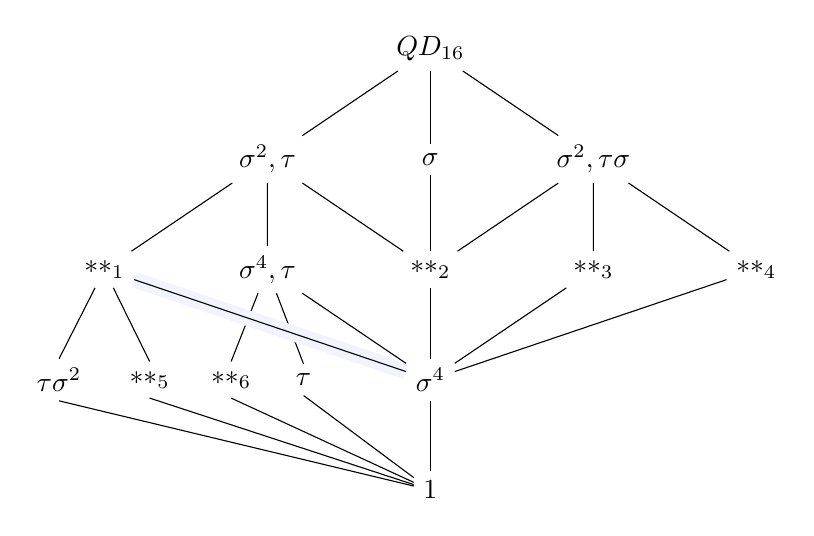
\begin{tikzpicture}[xscale=1.15, yscale=1.4]
            \node (G) at (0, 0) {$QD_{16}$};

            \node (s2t) at (-1.8, -1) {$\gen{\sigma^2, \tau}$};
            \node (s) at (0, -1) {$\gen \sigma$};
            \node (s2ts) at (1.8, -1) {$\gen{\sigma^2, \tau\sigma}$};

            \node (u1) at (-3.6, -2) {$\gen{**}_1$};
            \node (s4t) at (-1.8, -2) {$\gen{\sigma^4, \tau}$};
            \node (u2) at (0, -2) {$\gen{**}_2$};
            \node (u3) at (1.8, -2) {$\gen{**}_3$};
            \node (u4) at (3.6, -2){$\gen{**}_4$};

            \node (ts2) at (-4.1, -3) {$\gen{\tau\sigma^2}$};
            \node (u5) at (-3.1, -3) {$\gen{**}_5$};
            \node (u6) at (-2.2, -3) {$\gen{**}_6$};
            \node (t) at (-1.4, -3){$\gen \tau$};
            \node (s4) at (0, -3) {$\gen{\sigma^4}$};

            \node (1) at (0, -4) {1};

            \draw (1) -- (ts2.south);
            \draw (ts2.north) -- (u1) -- (s2t) -- (G);
            \draw (1) -- (u5.south);
            \draw (u5.north) -- (u1);
            \draw (1) -- (u6.south);
            \draw (u6.north) -- (s4t) -- (s2t);
            \draw (1) -- (t.south);
            \draw (t.north) -- (s4t);
            \draw (1) -- (s4) -- (u2) -- (s) -- (G);
            \draw [preaction={draw, line width=2mm, color=RoyalBlue!7}] (s4) -- (u1);
            \draw (s4) -- (s4t);
            \draw (s4) -- (u3) -- (s2ts) -- (G);
            \draw (s4) -- (u4) -- (s2ts);
            \draw (u2) -- (s2t);
            \draw (u2) -- (s2ts);
        \end{tikzpicture}
    \end{center}
\end{exercise}

\begin{sol}
    The above has had subscripts added to distinguish the unknown subgroups. It is clear that $\gen{**}_2$ must be $\gen{\sigma^2}$ since it is the only subgroup contained in both $\gen \sigma$ and $\gen{\sigma^2, \tau}$. To find the other subgroups, we calculate the cyclic subgroups of the form $\gen{\tau\sigma^k}$:
    \begin{align*}
        \gen{\tau\sigma} & = \set{1, \tau\sigma, \sigma^4, \tau\sigma^5} & \gen{\tau\sigma^3} & = \set{1, \tau\sigma^3, \sigma^4, \tau\sigma^7} \\
        \gen{\tau\sigma^4} & = \set{1, \tau\sigma^4} & \gen{\tau\sigma^6} & = \set{1, \tau\sigma^6}
    \end{align*}
    It becomes clear that 6 must be $\gen{\tau\sigma^4}$, since the subgroup above contains both $\tau$ and $\sigma^4$. 3 and 4 must be $\gen{\tau\sigma}$ and $\gen{\tau\sigma^3}$ respectively, since $\gen{\sigma^2, \tau\sigma}$ both contain $\tau\sigma$ and $\sigma^2$ which multiply to $\tau\sigma^3$. Certainly, 1 cannot be $\gen{\tau\sigma^6}$ as it does not contain $\gen{\tau\sigma^2}$, so it must be 5. Then 1 must be $\gen{\tau\sigma^2, \sigma^4}$ as it contains both subgroups. Hence, the completed diagram is
    \begin{center}
        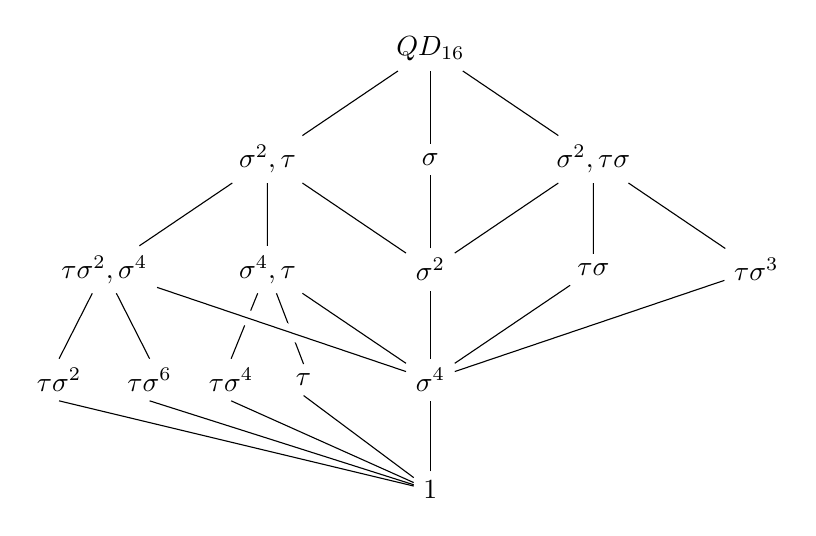
\begin{tikzpicture}[xscale=1.15, yscale=1.4]
            \node (G) at (0, 0) {$QD_{16}$};

            \node (s2t) at (-1.8, -1) {$\gen{\sigma^2, \tau}$};
            \node (s) at (0, -1) {$\gen \sigma$};
            \node (s2ts) at (1.8, -1) {$\gen{\sigma^2, \tau\sigma}$};

            \node (u1) at (-3.6, -2) {$\gen{\tau\sigma^2, \sigma^4}$};
            \node (s4t) at (-1.8, -2) {$\gen{\sigma^4, \tau}$};
            \node (u2) at (0, -2) {$\gen{\sigma^2}$};
            \node (u3) at (1.8, -2) {$\gen{\tau\sigma}$};
            \node (u4) at (3.6, -2){$\gen{\tau\sigma^3}$};

            \node (ts2) at (-4.1, -3) {$\gen{\tau\sigma^2}$};
            \node (u5) at (-3.1, -3) {$\gen{\tau\sigma^6}$};
            \node (u6) at (-2.2, -3) {$\gen{\tau\sigma^4}$};
            \node (t) at (-1.4, -3){$\gen \tau$};
            \node (s4) at (0, -3) {$\gen{\sigma^4}$};

            \node (1) at (0, -4) {1};

            \draw (1) -- (ts2.south);
            \draw (ts2.north) -- (u1) -- (s2t) -- (G);
            \draw (1) -- (u5.south);
            \draw (u5.north) -- (u1);
            \draw (1) -- (u6.south);
            \draw (u6.north) -- (s4t) -- (s2t);
            \draw (1) -- (t.south);
            \draw (t.north) -- (s4t);
            \draw (1) -- (s4) -- (u2) -- (s) -- (G);
            \draw [preaction={draw, line width=2mm, white}] (s4) -- (u1);
            \draw (s4) -- (s4t);
            \draw (s4) -- (u3) -- (s2ts) -- (G);
            \draw (s4) -- (u4) -- (s2ts);
            \draw (u2) -- (s2t);
            \draw (u2) -- (s2ts);
        \end{tikzpicture}
    \end{center}
\end{sol}

\begin{exercise} \label{ex2.5.12} 
    The group $A = Z_2 \times Z_4 = \gen{a, b \mid a^2 = b^4 = 1, ab = ba}$ has order 8 and has three subgroups of order 4: $\gen{a, b^2} \cong V_4, \gen b \cong Z_4$, and $\gen{ab} \cong Z_4$ and every proper subgroup is contained in one of these three. Draw the lattice of all subgroups of $A$, giving each subgroup in terms of at most two generators.
\end{exercise}

\begin{sol}
    Observe that $A$ is the direct product of two abelian groups, so $A$ is abelian, and we may write it as
    \[A = \set{1, a, b, b^2, b^3, ab, ab^2, ab^3}\]
    We know that $A$ has three subgroups of order 4: $\gen{a, b^2}, \gen b$, and $\gen{ab}$. To find what the containment relations are, observe that $\gen{a, b}^2$ has three subgroups of order 2: $\gen{b^2}, \gen a$, and $\gen{ab^2}$. $\gen b$ has the single subgroup of order 2: $\gen{b^2}$, and $\gen{ab}$ has the single subgroup of order 2: $\gen{ab^2}$. Then the subgroup lattice of $A$ is
    \begin{center}
        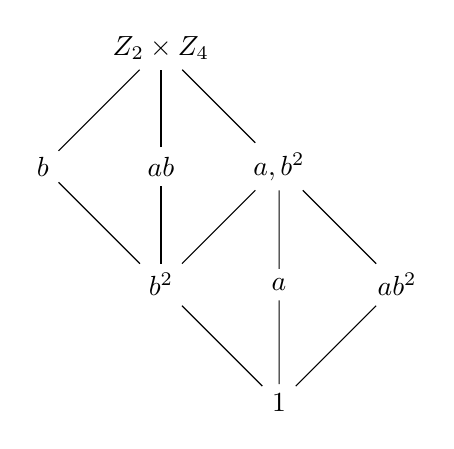
\begin{tikzpicture}[scale=1.5]
            \node (A) at (0, 0) {$Z_2 \times Z_4$};
            
            \node (b) at (-1, -1) {$\gen b$};
            \node (ab) at (0, -1) {$\gen{ab}$};
            \node (a b2) at (1, -1) {$\gen{a, b^2}$};

            \node (b2) at (0, -2) {$\gen{b^2}$};
            \node (a) at (1, -2) {$\gen a$};
            \node (ab2) at (2, -2) {$\gen{ab^2}$};

            \node (1) at (1, -3) {1};

            \draw (1) -- (b2) -- (b) -- (A);
            \draw (1) -- (a) -- (a b2) -- (A);
            \draw (b2) -- (ab) -- (A);
            \draw (b2) -- (a b2);
            \draw (1) -- (ab2) -- (a b2);
        \end{tikzpicture}
    \end{center}
\end{sol}

\begin{exercise} \label{ex2.5.13}
    The group $G = Z_2 \times Z_8 = \gen{x, y \mid x^2 = y^8 = 1, xy = yx}$ has order 16 and has three subgroups of order 8: $\gen{x, y^2} \cong Z_2 \times Z_4, \gen y \cong Z_8$, and $\gen{xy} \cong Z_8$, and every proper subgroup is contained in one of those three. Draw the lattice of all subgroups of $G$, giving each subgroups in terms of at most two generators (cf. \hyperref[ex2.5.12]{Exercise 2.5.12}).
\end{exercise}

\begin{sol}
    Let $x = a$ and $y^2 = b$, where $a$ and $b$ are the generators from \hyperref[ex2.5.12]{Exercise 2.5.12}. It follows that $G$ contains a copy of $Z_2 \times Z_4$ as $\gen{x, y^2} = \gen{a, b}$. Moreover, we may append $\gen y$ and $\gen{xy}$ to this lattice as follows:
    \begin{center}
        \begin{tikzpicture}[scale = 1.5]
            \node (G) at (0, 0) {$G$};

            \node (y) at (-1, -1) {$\gen y$};
            \node (xy) at (0, -1) {$\gen{xy}$};
            \node (x y2) at (1, -1) {$\gen{x, y^2}$};

            \node (y2) at (0, -2) {$\gen{y^2}$};
            \node (xy2) at (1, -2) {$\gen{xy^2}$};
            \node (x y4) at (2, -2) {$\gen{x, y^4}$};

            \node (y4) at (1, -3) {$\gen{y^4}$};
            \node (x) at (2, -3) {$\gen x$};
            \node (xy4) at (3, -3) {$\gen{xy^4}$};

            \node (1) at (2, -4) {1};

            \draw (1) -- (y4) -- (y2) -- (y) -- (G);
            \draw (1) -- (xy4) -- (x y4) -- (x y2) -- (G);
            \draw (1) -- (x) -- (x y4);
            \draw (y4) -- (xy2) -- (x y2);
            \draw (y2) -- (xy) -- (G);
            \draw (y4) -- (x y4);
            \draw (y2) -- (x y2);
        \end{tikzpicture}
    \end{center}
\end{sol}

\begin{exercise} \label{ex2.5.14} 
    Let $M$ be the group of order 16 with the following presentation:
    \[\gen{u, v \mid u^2 = v^8 = 1, vu = uv^5}\]
    (sometimes called the \textit{modular} group of order 16). It has three subgroups of order 8: $\gen{u, v^2}, \gen v$, and $\gen{uv}$, and every proper subgroup is contained in one of those three. Prove that $\gen{u, v^2} \cong Z_2 \times Z_4, \gen v \cong Z_8$, and $\gen{uv} \cong Z_8$. Show that the lattice of subgroups of $M$ is the same as the lattice of subgroups of $Z_2 \times Z_8$ (cf. Exercise 13) but that these two groups are not isomorphic.
\end{exercise}

\begin{sol}
    It is clear that $\abs v = 8$ implies that $\gen v \cong Z_8$. Similarly, since $\abs{uv} = 8$, then $\gen{uv} \cong Z_8$. To see that $\gen{u, v^2} \cong Z_2 \times Z_4$, we verify the relations. Note that $u^2 = (v^2)^4 = 1$, and
    \[v^2u = vuv^5 = uv^{10} = uv^2\]
    so that $u$ and $v^2$ commute, hence it is abelian. We may then list out the elements of $\gen{u, v^2}$:
    \[\gen{u, v^2} = \set{1, v^2, v^4, v^6, u, uv^2, uv^4, uv^6}\]
    Then the mapping $\phi : Z_2 \times Z_4 \to \gen{u, v^2}$ defined by
    \[\phi(a) = u, \quad \phi(b) = v^2\]
    extends to a homomorphism. Moreover, it is clear that distinct elements in $Z_2 \times Z_4$ map to distinct elements in $\gen{u, v^2}$, so that $\phi$ is injective. As shown above, $|\gen{u, v^2}| = 8 = |Z_2 \times Z_4|$, so that $\phi$ is surjective. Hence, $\phi$ is an isomorphism and $Z_2 \times Z_4 \cong \gen{u, v^2}$. The subgroup lattice of $M$ is then the same as that of $Z_2 \times Z_8$ as shown in \hyperref[ex2.5.13]{Exercise 2.5.13}, but with $u = x$ and $v = y$:
    \begin{center}
        \begin{tikzpicture}[scale = 1.5]
            \node (G) at (0, 0) {$G$};

            \node (y) at (-1, -1) {$\gen v$};
            \node (xy) at (0, -1) {$\gen{uv}$};
            \node (x y2) at (1, -1) {$\gen{u, v^2}$};

            \node (y2) at (0, -2) {$\gen{v^2}$};
            \node (xy2) at (1, -2) {$\gen{uv^2}$};
            \node (x y4) at (2, -2) {$\gen{u, v^4}$};

            \node (y4) at (1, -3) {$\gen{v^4}$};
            \node (x) at (2, -3) {$\gen u$};
            \node (xy4) at (3, -3) {$\gen{uv^4}$};

            \node (1) at (2, -4) {1};

            \draw (1) -- (y4) -- (y2) -- (y) -- (G);
            \draw (1) -- (xy4) -- (x y4) -- (x y2) -- (G);
            \draw (1) -- (x) -- (x y4);
            \draw (y4) -- (xy2) -- (x y2);
            \draw (y2) -- (xy) -- (G);
            \draw (y4) -- (x y4);
            \draw (y2) -- (x y2);
        \end{tikzpicture}
    \end{center}
    Finally, $M$ is not isomorphic to $Z_2 \times Z_8$ since $M$ is not abelian. If it were, then $vu = uv$, but $vu = uv^5 = uv$ would imply that $v^4 = 1$, contradicting that $\abs v = 8$.
\end{sol}

\newpage

\begin{exercise}
    Describe the isomorphism type of each of the three subgroups of $D_{16}$ of order 8.
\end{exercise}

\begin{sol}
    Since $\abs r = 8$, then $\gen r \cong Z_8$. For the remaining subgroups, note that the lattice for $D_{16}$ shows a striking similarity to the lattice for $D_8$; in fact, these subgroups \textit{are} isomorphic to $D_8$ as follows:
    
    For the subgroup $\gen{s, r^2}$, observe that $(r^2)4 = s^2 = 1$, and $sr^2 = r^6s = (r^2)\inv s$. Then the mapping $\phi : D_8 \to \gen{s, r^2}$ given by
    \[\phi(r) = r^2, \quad \phi(s) = s\]
    extends to a homomorphism. Moreover, this mapping is surjective by construction. Since $\gen{s, r^2}$ contains a subgroup of order 4 and is a subgroup of $D_{16}$, it must be 8 so that $\phi$ is an isomorphism, and $D_8 \cong \gen{s, r^2}$.
    
    For the subgroup $\gen{sr, r^2}$, we again observe that $(r^2)^4 = (sr)^2 = 1$, and $(sr)r^2 = sr^3 = r^5s = r^6r^7s = (r^2)\inv(sr)$. The mapping $\psi : D_8 \to \gen{sr, r^2}$ given by
    \[\phi(r) = r^2, \phi(s) = sr\]
    extends to a homomorphism, surjective by construction, and is an isomorphism because $\gen{sr, r^2}$ has order 8. Then $D_8 \cong \gen{sr, r^2}$.
\end{sol}

\begin{exercise}
    Use the lattice of subgroups of the quasidihedral of order 16 to show that every element of order 2 is contained in the proper subgroup $\gen{\tau, \sigma^2}$ (cf. \hyperref[ex2.5.11]{Exercise 2.5.11}).
\end{exercise}

\begin{sol}
    Every element of order 2 generates a cyclic subgroup of order 2. Using the lattice, $\gen{\tau, \sigma^2}$ properly contains all cyclic subgroups, except $\gen{\tau\sigma}$ and $\gen{\tau\sigma^3}$, both of which are order 4. Then $\gen{\tau, \sigma^2}$ contains all cyclic subgroups of order 2, hence contain all elements of order 2.
\end{sol}

\begin{exercise}
    Use the lattice of subgroups of the modular group $M$ of order 16 to show that the set $\set{x \in M \mid x^2 = 1}$ is a subgroup of $M$ isomorphic to the Klein 4-group (cf. \hyperref[ex2.5.14]{Exercise 2.5.14}).
\end{exercise}

\begin{sol}
    Using the lattice in Exercise 14, we see that we have 3 candidates to be isomorphic to $V_4$, namely $\gen{v^2}, \gen{uv^2},$ and $\gen{u, v^4}$. The first and second subgroups are cyclic, while $\gen{u, v^4} = \set{1, u, v^4, uv^4}$. Since it is not generated by one element, each of these elements are of order 2, and $v^4u = v^3uv^5 = \cdots = uv^{20} = uv^4$ so that it is abelian, then $\gen{u, v^4} \cong V_4$.
\end{sol}

\begin{exercise}
    Use the lattice to help find the centralizer of every element of $QD_{16}$ (cf. \hyperref[ex2.5.11]{Exercise 2.5.11}).
\end{exercise}

\begin{sol}
    Note that $\sigma^4\tau = \sigma^3\tau\sigma^3 = \cdots = \tau\sigma^{12} = \tau\sigma^4$ so that $\sigma^4 \in Z(QD_{16})$ as $\sigma^4$ already commutes with powers of $\sigma$. Moreover, any power of $\sigma$ does not commute with $\tau$ except for $\sigma^4$. The elements $\tau\sigma$ and $\tau\sigma^3$ do not commute with $\sigma^2$ as $(\tau\sigma)\sigma^2 = \tau\sigma^3 = \sigma\tau \neq \sigma^2(\tau\sigma) = \tau\sigma^2$, and $(\tau\sigma^3)\sigma^2 = \sigma^7\tau \neq \sigma^3\tau = \sigma^2(\tau\sigma^3)$. Next, $(\tau\sigma^2)\sigma^2 = \tau\sigma^4 \neq \tau = \sigma^2(\tau\sigma^2)$ so that $\sigma^2$ does not commute with $\tau\sigma^2$. Moreover, $(\tau\sigma^6)(\tau\sigma^2) = \tau\sigma^2\sigma^4\tau\sigma^2 = (\tau\sigma^2)(\tau\sigma^6)$ so that $\tau\sigma^2$ commutes with $\tau\sigma^6$, but $\sigma^2\tau\sigma^6 = \tau\sigma^4 \neq \tau = (\tau\sigma^6)\sigma^2$ so $\sigma^2$ does not commute with $\tau\sigma^6$. Lastly, $\sigma^2(\tau\sigma^4) = \tau\sigma^2 \neq (\tau\sigma^4)\sigma^2$, and $\sigma^2\tau = \tau\sigma^6 \neq \tau\sigma^2$ so that $\sigma^2$ does not commute with $\tau\sigma^4$ nor with $\tau$. It follows that the centralizers of the elements of $QD_{16}$ are
    \begin{align*}
        C_{QD_{16}}(1) = C_{QD_{16}}(\sigma^4) & = QD_{16} \\
        C_{QD_{16}}(\gen{\sigma^k}) & = \gen\sigma \text{ for $k = 1, 2, 3, 5, 6, 7$} \\
        C_{QD_{16}}(\gen{\tau\sigma}) = C_{QD_{16}}(\gen{\tau\sigma^5}) & = \gen{\tau\sigma} \\
        C_{QD_{16}}(\gen{\tau\sigma^3}) = C_{QD_{16}}(\gen{\tau\sigma^7}) & = \gen{\tau\sigma^3} \\
        C_{QD_{16}}(\gen\tau) = C_{QD_{16}}(\gen{\tau\sigma^4}) & = \gen{\sigma^4, \tau} \\
        C_{QD_{16}}(\gen{\tau\sigma^2}) = C_{QD_{16}}(\gen{\tau\sigma^6}) & = \gen{\tau\sigma^2, \sigma^4}
    \end{align*}
\end{sol}

\begin{exercise}
    Use the lattice to help find $N_{D_{16}}(\gen{s, r^4})$.
\end{exercise}

\begin{sol}
    Based on the placement of $\gen{s, r^4}$, its normalizer may be itself, $\gen{s, r^2}$, or $D_{16}$. Note that $\gen{s, r^4} = \{1, s, r^4, sr^4\}$, and taking $r^2$ and $(r^2)\inv = r^6$, we have
    \[r^2\gen{s, r^4}r^6 = \set{1, sr^4, r^4, s} = \gen{s, r^4}\]
    so that $r^2 \in N_{D_{16}}(\gen{s, r^4})$, and $\gen{s, r^2} \leq N_{D_{16}}(\gen{s, r^4})$. Since $rsr\inv = r^2s \neq r$, then $r \not\in N_{D_{16}}(\gen{s, r^4})$ so that $N_{D_{16}}(\gen{s, r^4}) = \gen{s, r^2}$.
\end{sol}

\begin{exercise}
    Use the lattice of subgroups of $QD_{16}$ (cf. \hyperref[ex2.5.11]{Exercise 2.5.11}) to help find the normalizers
    \begin{subproblems}
        \item $N_{QD_{16}}(\gen{\tau\sigma})$ \quad (b)~~$N_{QD_{16}}(\gen{\tau, \sigma^4})$.
    \end{subproblems}
\end{exercise}

\begin{solalph}
    \item Note that $\gen{\tau\sigma} = \set{1, \tau\sigma, \sigma^4, \tau\sigma^5}$. Moreover, $(\sigma^2)\inv = \sigma^6$ so that
    \[\sigma^2\gen{\tau\sigma}\sigma^6 = \{1, \tau\sigma^4, \sigma^4, \tau\sigma\} = \gen{\tau\sigma}\]
    and $\sigma(\tau\sigma)\sigma^7 = \tau\sigma^3 \neq \tau\sigma$ so that $\sigma \not\in N_{QD_{16}}(\gen{\tau\sigma})$. Then $N_{QD_{16}}(\gen{\tau\sigma}) = \gen{\sigma^2, \tau\sigma}$.
    \item $\gen{\tau, \sigma^4} = \{1, \tau, \sigma^4, \tau\sigma^4\}$, and 
    \[\sigma^2\gen{\tau, \sigma^4}\sigma^6 = \{1, \tau\sigma^4, \sigma^4, \tau\}\]
    while $\sigma\tau\sigma^7 = \tau\sigma^2 \neq \tau$ so that $\sigma \not\in N_{QD_{16}}(\gen{\tau, \sigma^4})$. Then $N_{QD_{16}}(\gen{\tau, \sigma^4}) = \gen{\sigma^2, \tau}$.
\end{solalph}